\documentclass[a4paper,12pt]{report}
\usepackage[top=1.5cm]{geometry}
\usepackage{natbib}
\usepackage{url}
\usepackage{titlesec}
\usepackage{graphicx}
\usepackage{pifont}
\usepackage{pgfmath}
\usepackage{hyperref}
\usepackage{multirow}
\usepackage{hhline}
\usepackage{tabularx}
\usepackage{cellspace}
\usepackage{array}
\usepackage{colortbl}
\usepackage[table]{xcolor}

\setcounter{secnumdepth}{3} 

\titleformat{\chapter}[hang]{\normalfont\bfseries}{\thechapter.}{1em}{}
\titleformat{\section}[hang]{\normalfont\bfseries}{\thesection.}{1em}{}
\titleformat{\subsection}[hang]{\normalfont\bfseries}{\thesubsection.}{0.5em}{}
\titleformat{\subsubsection}[hang]{\normalfont\bfseries}{\thesubsubsection.}{0.5em}{}
\titlespacing{\chapter}{0pt}{-1cm}{1cm}
\titlespacing{\section}{0pt}{0.5cm}{0.2cm}
\titlespacing{\subsection}{0pt}{0.3cm}{0.1cm}
\titlespacing{\subsubsection}{0pt}{0.6cm}{0.2cm}



\begin{document}

\begin{titlepage}
    \begin{center}
        \textbf{\Large PONTIFÍCIA UNIVERSIDADE CATÓLICA DE MINAS GERAIS}

        \vspace{0.5cm}

        \textbf{\Large PUC Minas Virtual}
        
        \vspace{2cm}
        
        \textbf{\Large Pós-Graduação Lato Sensu em Arquitetura de Software Distribuído}
        
        \vspace{2cm}
        
        \textbf{\Large Projeto Integrado}
        
        \vspace{0.5cm}
        
        \textbf{\Large Relatório Técnico}

        \vspace{1cm}

        \textbf{\Large Sistema de Gestão de Delivery}
        
        \vspace{4cm}
        
        \textbf{\Large Julio Cezar da Silva}
        
        \vspace{4cm}
        
        \textbf{\Large Belo Horizonte}\\
        \textbf{\Large 2023}
    \end{center}
    
    \newpage
    \thispagestyle{empty}
    
    \begin{center}
        \textbf{\Large Julio Cezar da Silva}
    \end{center}
    
    \vspace{4cm}
    
    \begin{center}
        \textbf{\Large Sistema de Gestão de Delivery}
    \end{center}
    
    \vspace{1cm}
    
    \begin{flushright}
        Trabalho de Conclusão de Curso de Especialização em Arquitetura de Software Distribuído como requisito parcial à obtenção do título de especialista.
    \end{flushright}
    
    \vspace{4cm}
    
    \begin{flushleft}
        Orientador: Prof. Luiz Alberto
    \end{flushleft}
    
    \vspace{2cm}
    
    \begin{center}
        \textbf{\Large Belo Horizonte}\\
        \textbf{\Large 2023}
    \end{center}
    
\end{titlepage}


\renewcommand{\contentsname}{Sumário}
\tableofcontents
\chapter{Introdução}
O mercado de delivery tem crescido de forma significativa no Brasil, o mesmo foi impulsionado ainda mais 
devido a pandemia de COVID-19. 

Segundo a Associação brasileira de Bares e Restaurantes(Abrasel), o setor de alimentação movimentou cerca
de R\$ 200 bilhões em 2019, sendo que destes, 11\% foi representado pelo delivery. Em 2020 com a pandemia, o
mercado cresceu para 20\% do faturamento total do setor\cite{abraselexpansao}.

Durante a pandemia tivemos um grande aumento no uso de plataformas de delivery, principalmente
do ifood\cite{ifoodprincipal} que hoje é a principal plataforma de delivery no Brasil. Essas plataformas possuem
uma taxa altíssima, mesmo as altas taxas aplicadas, que variam de 12\% a 27\%, além de uma
mensalidade em torno de R\$ 100,00\cite{ifoodtaxa}.

De acordo com o Instituto FoodService Brasil(IFB), no Brasil espera-se que o delivery cresça em torno de 7,5\% em 2023,
fazendo com que os estabelecimentos invistam em ampliar e aprimorar este serviço de entrega de comida\cite{ifb2023}.

A transformação digital\cite{transformacaodigital} está presente nas nossas atividades diárias, e não está limitada ao uso pessoal, o setor 
de delivery está cada vez mais preparado digitalmente, e os estabelecimentos que não adotarem as tecnologias que 
possam facilitar seus processos, controles e integração com os clientes ficarão para trás no mercado. 

Com a utilização de tecnologias como sistemas gerenciais, o estabelecimento evita e minimiza erros e prejuízos nos 
seus processos, tem um melhor controle de estoque, financeiro e diversas rotinas do seu comércio. Além de otimizar
o tempo tanto de preparação com as comandas chegando automáticamente via sistema, sem a movimentação de papel que 
pode se perder no processo, quanto a agilidade em atender o cliente e cadastrar seu pedido, algo que pode ser inclusive
feito pelo próprio cliente direto de sua casa.
\chapter{Objetivo}

O objetivo do projeto é apresentar uma arquitetura de um sistema para estabelecimentos de alimentação, de modo
que os mesmos possam ter um controle dos seus produtos, clientes e da sua rotina. Além de um sistema que permita
aos clientes efetuarem pedidos de forma online.

Portanto, com objetivo de desenvolver a modelagem de um software no qual os estabelecimentos possam utilizar e 
oferecer através do mesmo diversos benefícios aos seus clientes, como promoções, fidelização do cliente,
mensagens diretas ao smartphone do cliente, até mesmo preços mais baixos desde que o estabelecimento faça um bom marketing para 
atrair clientes que utilizem plataformas de pedidos como ifood.

O cliente poderá acessar o software através de um aplicativo para smartphone, seja uma progressive
web page, ou mesmo um aplicativo nativo, o que será definido no decorrer das análises e projeto arquitetural.

\section{Objetivos Específicos}
Os objetivos específicos são:

\begin{itemize}
    \item Permitir ao estabelecimento ter um controle dos seus cadastros de clientes, produtos, promoções, etc.
    \item Oferecer ao cliente do estabelecimento um sistema facilitador para que o mesmo possa efetuar pedidos diretamente da sua casa.
    \item Facilitar ao estabelecimento oferecer promoções diretamente ao cliente em casa, através do próprio sistema, isto é, enviar promoções para o cliente, 
    mensagens de aniversário ou que mais convier ao estabelecimento.
    \item Facilitar o controle de estoque do estabelecimento. 
    \item Facilitar o controle financeiro do estabelecimento.
    \item Permitir o fácil gerenciamento do estabelecimento através de diversos relatorios.
    \item Oferecer ao cliente a opção de pagar online, para isso deverá ser feito integrações com os principais players de pagamento, como pagseguro, mercadopago, etc.
    \item Permitir ao estabelecimento receber pedidos de plataformas de delivery como ifood.
\end{itemize}


\chapter{Restrições Arquiteturais}

\begin{table}[h]
    \caption{Restrições}
    \centering
    \vspace{0.5cm}
    \resizebox{\textwidth}{!}{%
    \begin{tabular}{|c|p{10cm}|p{2cm}|p{2cm}|}
        \hline
        ID & Descrição \\ 
        \hline                               % para uma linha horizontal
        RA001 & O software deverá ser desenvolvido em Java utilizando o framwork Spring \\
        \hline
        RA002 & As APIs devem seguir o padrão RestFul \\
        \hline        
        RA003 & O software deverá integrar com com plataformas de delivery, de forma a permitir os clientes pedirem por ela, como ifood. \\
        \hline        
        RA004 & O software deverá integrar com pelo menos um sistema de pagamento online, como pagseguro, mercadopago. \\
        \hline  
        \hline        
        RA005 & O software administrativo do estabelecimento deverá ter níveis de acesso para proteger dados sensíveis,
        como endereço e outras informações pessoais dos clientes \\
        \hline              
    \end{tabular}%
    }
\end{table}
\pgfmathsetmacro\nreq{0}
\chapter{Requisitos Funcionais}
Abaixo listamos os requisitos funcionais da aplicação\cite{Sommerville:2011}.
Os requisitos terão níveis de dificuldade e prioridades definidos em B - Baixa, M - Média e A - Alta.

\section{Módulo de produtos}
\vspace{0.5cm}

\pgfmathtruncatemacro\nreq{\nreq + 1}
\subsection{RF-\nreq: Cadastro de produtos}
O sistema deve permitir que o colaborador cadastre produtos com nome, categoria, preço de custo por tamanho, preço de venda por tamanho, 
unidade de medida, descrição, foto, se será feito controle de estoque, ficha técnica, complementos.

\vspace{0.5cm}
\noindent\textbf{\textit{Dificuldade:}} \textit{M -} \textbf{\textit{Prioridade:}} \textit{A}
\vspace{0.5cm}
\pgfmathtruncatemacro\nreq{\nreq + 1}
\subsection{RF-\nreq: Cadastro de categoria}
O sistema deve permitir cadastrar a categoria de produtos, definindo possiveis tamanhos dos produtos nessa categoria ou tamanho únicoa, por exemplo: Refrigerantes, definir os 
tamanhos 350ml, 500ml, 1l, 1.5l, 2l, etc.

\vspace{0.5cm}
\noindent\textbf{\textit{Dificuldade:}} \textit{M -} \textbf{\textit{Prioridade:}} \textit{A}
\vspace{0.5cm}
\pgfmathtruncatemacro\nreq{\nreq + 1}
\subsection{RF-\nreq: Cadastro de complementos}
O sistema deverá permitir cadastrar complementos e seus valores, os mesmos deverão ser ligados ao tamanho do produto no cadastro de produtos.
Exemplo: Acrescimo de Bacon pizza M, Acrescimo de Bacon pizza G e assim por diante.

\vspace{0.5cm}
\noindent\textbf{\textit{Dificuldade:}} \textit{B -} \textbf{\textit{Prioridade:}} \textit{M}
\vspace{0.5cm}
\pgfmathtruncatemacro\nreq{\nreq + 1}
\subsection{RF-\nreq: Cadastro de combos}
O sistema deverá permitir o cadastro de combos, juntando vários produtos cadastrados em um combo e definindo o valor
para o combo.

\vspace{0.5cm}
\noindent\textbf{\textit{Dificuldade:}} \textit{A -} \textbf{\textit{Prioridade:}} \textit{M}
\vspace{0.5cm}

\section{Módulo de clientes}
\vspace{0.5cm}
\pgfmathtruncatemacro\nreq{\nreq + 1}
\subsection{RF-\nreq: Cadastro de clientes}
O sistema deve permitir cadastrar os clientes com nome, email, data nascimento, telefone principal, cpf ou cnpj, identidade ou 
inscrição estadual, endereço principal(endereço, número, complemento, bairro, cidade, cep, valor do frete).

\vspace{0.5cm}
\noindent\textbf{\textit{Dificuldade:}} \textit{B -} \textbf{\textit{Prioridade:}} \textit{A}
\vspace{0.5cm}

\pgfmathtruncatemacro\nreq{\nreq + 1}
\subsection{RF-\nreq: Cadastro de endereços de clientes}
O sistema deverá permitir cadastrar mais endereços para o cliente, com nome do endereço e os campos definidos no requisito RF-004.

\vspace{0.5cm}
\noindent\textbf{\textit{Dificuldade:}} \textit{B -} \textbf{\textit{Prioridade:}} \textit{M}
\vspace{0.5cm}

\section{Módulo de pedidos}
\vspace{0.5cm}
\pgfmathtruncatemacro\nreq{\nreq + 1}
\subsection{RF-\nreq: Cadastro de pedidos delivery}
O sistema deve permitir cadastrar pedidos para os clientes, selecionando cliente, produtos, endereço de entrega,
forma de pagamento, status do pedido(Aberto, Em preparo, Pronto/Para retirar, Saiu para Entregar, Finalizado/Entregue),
lançamento de desconto ou taxa de serviço.

\vspace{0.5cm}
\noindent\textbf{\textit{Dificuldade:}} \textit{A -} \textbf{\textit{Prioridade:}} \textit{A}
\vspace{0.5cm}

\pgfmathtruncatemacro\nreq{\nreq + 1}
\subsection{RF-\nreq: Cadastro de pedidos mesa}
O sistema deve permitir cadastrar pedidos para os clientes no estabelecimento, selecionando cliente, produtos, 
forma de pagamento, status do pedido(Aberto, Em preparo, Pronto/Para retirar, Saiu para Entregar, Finalizado/Entregue),
lançamento de desconto ou taxa de serviço, divisão de valores.

\vspace{0.5cm}
\noindent\textbf{\textit{Dificuldade:}} \textit{A -} \textbf{\textit{Prioridade:}} \textit{A}
\vspace{0.5cm}

\pgfmathtruncatemacro\nreq{\nreq + 1}
\subsection{RF-\nreq: Cadastro de pedidos cliente}
O sistema deve permitir que o próprio cliente faça seu pedido online, selecionando os produtos, endereço de entrega.

\vspace{0.5cm}
\noindent\textbf{\textit{Dificuldade:}} \textit{A -} \textbf{\textit{Prioridade:}} \textit{A}
\vspace{0.5cm}

\section{Módulo de estoque}
\vspace{0.5cm}
\pgfmathtruncatemacro\nreq{\nreq + 1}
\subsection{RF-\nreq: Cadastro de ingredientes}
O sistema deve permitir o gerenciamento do estoque através do cadastro de ingredientes, e nos produtos que 
controlam estoque ter a ficha técnica dos mesmos ligadas aos ingredientes. O cadastro deverá ter informações
como nome do ingrediente, unidade de medida, data de vencimento, preço de custo.

\vspace{0.5cm}
\noindent\textbf{\textit{Dificuldade:}} \textit{A -} \textbf{\textit{Prioridade:}} \textit{M}
\vspace{0.5cm}
\pgfmathtruncatemacro\nreq{\nreq + 1}
\subsection{RF-\nreq: Relatório de estoque}
O sistema deve possuir relatorio que mostre o estoque de produtos e os produtos com vencimento próximo, de modo a 
evitar perdas.

\vspace{0.5cm}
\noindent\textbf{\textit{Dificuldade:}} \textit{A -} \textbf{\textit{Prioridade:}} \textit{M}
\vspace{0.5cm}

\section{Módulo financeiro}
\vspace{0.5cm}
\pgfmathtruncatemacro\nreq{\nreq + 1}
\subsection{RF-\nreq: Formas de pagamento}
O sistema deve permitir o gerenciamento das formas de pagamento, para que possam ser selecionadas no lançamento do
pedido. Exemplo: Cartão de Credito, Cartão de Débito, Dinheiro, Pix, etc. Também as respectivas bandeiras quando 
necessário.

\vspace{0.5cm}
\noindent\textbf{\textit{Dificuldade:}} \textit{A -} \textbf{\textit{Prioridade:}} \textit{M}
\vspace{0.5cm}
\pgfmathtruncatemacro\nreq{\nreq + 1}
\subsection{RF-\nreq: Pagamento Online}
O sistema deve fazer integração com pelo menos 1 meio de pagamento online como pagseguro ou mercado pago.

\vspace{0.5cm}
\noindent\textbf{\textit{Dificuldade:}} \textit{A -} \textbf{\textit{Prioridade:}} \textit{B}
\vspace{0.5cm}

\section{Módulo autenticação/autorização}
\vspace{0.5cm}
\pgfmathtruncatemacro\nreq{\nreq + 1}
\subsection{RF-\nreq: Níveis de acesso}
O sistema deve permitir o cadastro/gerenciamento de níveis de acesso, a principio dois níveis serão suficientes: Usuário e 
Administrador.
Os usuários poderão fazer lançamento de pedidos, cadastros de clientes.
Os administradores terão acesso irrestrito ao sistema.

\vspace{0.5cm}
\noindent\textbf{\textit{Dificuldade:}} \textit{B -} \textbf{\textit{Prioridade:}} \textit{A}
\vspace{0.5cm}

\pgfmathtruncatemacro\nreq{\nreq + 1}
\subsection{RF-\nreq: Autenticação}
O sistema deve ser fechado, não permitido o acesso a ele, somente para usuários cadastrados através de autenticação.
Clientes externos deverão poder acessar um cardápio online e ao efetuar pedido fazer o devido cadastro.

\vspace{0.5cm}
\noindent\textbf{\textit{Dificuldade:}} \textit{A -} \textbf{\textit{Prioridade:}} \textit{A}
\vspace{0.5cm}


\pgfmathsetmacro\nreqnf{0}
\chapter{Requisitos Não Funcionais}
Abaixo listamos os requisitos não funcionais da aplicação em termos arquiteturais\cite{Sommerville:2011}.

\section{Manutenabilidade}
\vspace{0.5cm}
\pgfmathtruncatemacro\nreqnf{\nreqnf + 1}
\subsection{RNF-\nreqnf: Desenvolvimento em camadas}
O sistema deve ser desenvolvido utilizando uma arquitetura em camadas, de modo a facilitar a manutenção do mesmo. A principio
podemos utilizar o modelo MVC(Model View Controller).

\vspace{0.5cm}
\noindent\textbf{\textit{Prioridade:}} \textit{M}

\vspace{0.5cm}
\section{Usabilidade}
\pgfmathtruncatemacro\nreqnf{\nreqnf + 1}
\subsection{RNF-\nreqnf: Padrão de interfaces}
O sistema deve ser desenvolvido de modo a manter um padrão na interface com o usuário, de modo a facilitar 
a famializariação do usuário com as telas do sistema. O sistema deverá funcionar também de 
maneira responsiva, de modo a ser fácil de se utilizar em dispositivos móveis quanto em computadores.  

\vspace{0.5cm}
\noindent\textbf{\textit{Prioridade:}} \textit{A}
\vspace{0.5cm}
\section{Segurança}
\pgfmathtruncatemacro\nreqnf{\nreqnf + 1}
\subsection{RNF-\nreqnf: Banco de dados}
O sistema deve proteger os dados sensíveis dos clientes e usuários através de criptografia de senhas no banco de dados,
acesso restrito ao banco de dados, o mesmo não deverá ter acesso externo a internet. 

\vspace{0.5cm}
\noindent\textbf{\textit{Prioridade:}} \textit{A}
\pgfmathtruncatemacro\nreqnf{\nreqnf + 1}
\vspace{0.5cm}
\subsection{RNF-\nreqnf: Autenticação/Autorização}
O sistema deverá ter mecanismos de autenticação e autorização para somente determinados níveis acessar informações mais sensíveis.  

\vspace{0.5cm}
\noindent\textbf{\textit{Prioridade:}} \textit{A}
\vspace{0.5cm}
\section{Interoperabilidade}
\pgfmathtruncatemacro\nreqnf{\nreqnf + 1}
\subsection{RNF-\nreqnf: Comunicação com sistema de pagamento}
O sistema deve ser capaz de se comunicar/integrar com pelo menos um meio de pagamento externo como pagseguro através de uma API.  

\vspace{0.5cm}
\noindent\textbf{\textit{Prioridade:}} \textit{M}
\vspace{0.5cm}
\section{Desempenho}
\pgfmathtruncatemacro\nreqnf{\nreqnf + 1}
\subsection{RNF-\nreqnf: Acesso após Autenticação}
O sistema deve ser capaz de exibir sua tela inicial após a inserção dos dados de acesso em menos de 5 segundos.  

\vspace{0.5cm}
\noindent\textbf{\textit{Prioridade:}} \textit{M}
\vspace{0.5cm}
\pgfmathsetmacro\nreqnf{0}
\chapter{Mecanismos Arquiteturais}
Abaixo listamos os mecanismos que irão compor a arquitetura do software proposto.
\begin{table}[h]
    \caption{Módulo Cadastros}

    \vspace{0.5cm}
    \resizebox{\textwidth}{!}{
    \begin{tabular}{|l|p{6cm}|p{6cm}|}
        \hline
        Análise & Design & Implementação \\ % Note a separação de col. e a quebra de linhas
        \hline                               % para uma linha horizontal
        Mapeamento objeto-relacional & Utilização do padrão de projeto Data Access Object (DAO) & Utilização do Hibernate como framework ORM \\      
        \hline      
        Gerenciamento de dados estruturados & Modelagem de banco de dados relacional & Utilização do PostgreSQL como SGBD \\      
        \hline    
        Autenticação de usuários &  Utilização de algoritmo de criptografia unidirecional para armazenamento de senhas, como SHA-256 ou bcrypt, e implementação de um mecanismo de validação de login e senha no servidor. & Utilização de um framework de autenticação, como Spring Security \\      
        \hline   
        Integração entre diferentes sistemas &  Utilização de protocolos e formatos de dados interoperáveis, como JSON & Utilização de APIs RESTful para comunicação entre os sistemas.\\      
        \hline  
        Registro de atividades do sistema (log) & Utilização de frameworks de logging &  Log4j \\      
        \hline
        Gerenciamento de versões de código & Utilização de um sistema de controle de versão &  GitHub \\      
        \hline
        Documentação das APIs & Utilização ferramentas de documentação &  Swagger \\      
        \hline   
        Teste do Software & Utilização de testes unitários, trabalhar com a metodologia TDD &  JUnit \\      
        \hline
        Front-end & Interface de comunicação com o usuário do sistema &  Angular \\      
        \hline   
        Back-end & Utilização de arquitetura MVC e injeção de dependências &  Spring framework \\      
        \hline                                
    \end{tabular}
    }
\end{table}

\chapter{Modelagem Arquitetural}

Apresentamos abaixo a modelagem arquitetural do sistema de delivery, utilizaremos para nossa modelagem o modelo C4.

\section{Diagrama de Contexto}
Começaremos pelo diagrama de contexto, nele temos o nosso sistema de delivery Pop Food que é
responsável por gerenciar todo o estabelecimento, e os atores como clientes e atendentes/administradores que fazem pedido de comida
e são responsáveis pela administração dentro do software respectivamente. Podemos verificar ainda 
os sistemas externos como PagSeguro e Ifood para pagamento e pedidos online respectivamente.
\begin{figure}[h]
  \centering
  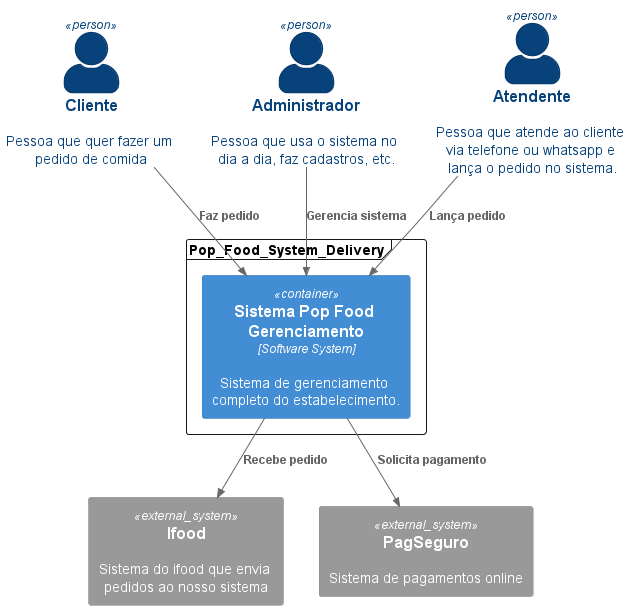
\includegraphics[width=1\textwidth]{diagrama_contexto.png}
  \caption{Diagrama de Contexto}
  \label{fig:Diagrama de Contexto}
\end{figure}

  \href{https://github.com/soltein/TCC/blob/main/Diagramas/out/diagrama_contexto/diagrama_contexto.png}{Imagem resolução maior}

  \section{Diagrama de Container}
  Mostramos agora o diagrama de container, nele podemos observar que teremos dois containers de frontend,
  ambos utilizando a tecnologia Angular, o frontend do Cliente é responsável por apresentar as telas do sistema
  que os clientes utilizarão para se cadastrar, ver o menu de opções, efetuar pedidos e pagamentos online.

  No frontend de administração será disponibilizado as telas de login e administração do sistema, como cadastro de produtos, possibilidade de lançamento de pedidos,
  cadastro de clientes, etc.

  Neste diagrama vemos o container do back end, que utilizará spring boot e será responsável pelas regras de negócio e integração com banco de dados e sistemas externos como iFood e PagSeguro.

  \begin{figure}[h]
    \centering
    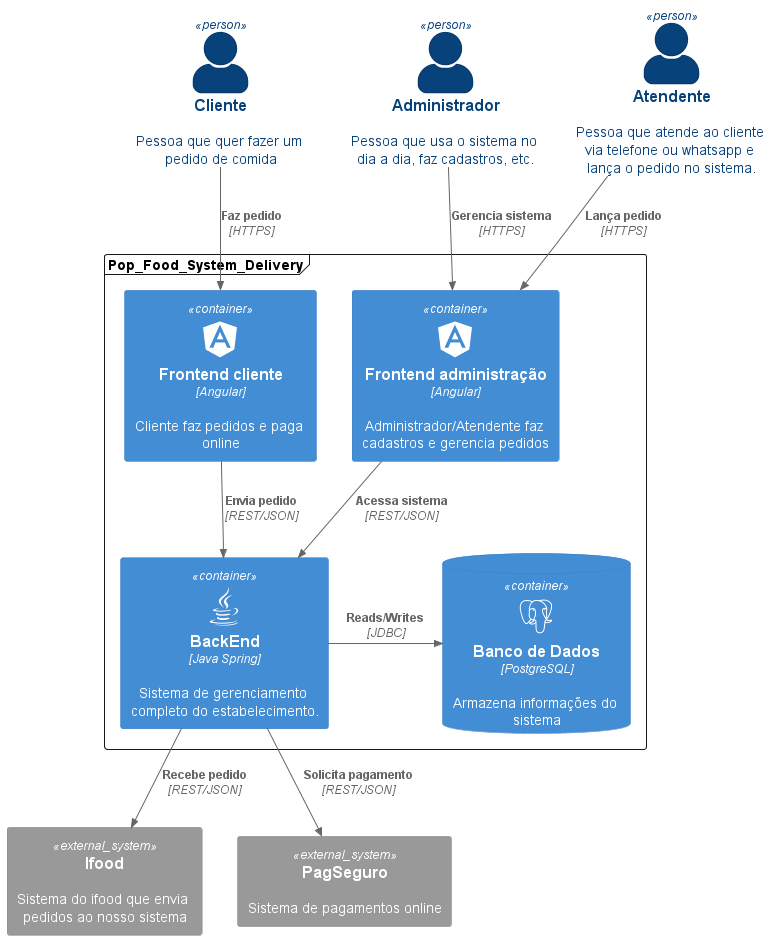
\includegraphics[width=0.9\textwidth]{diagrama_container.png}
    \caption{Diagrama de Container}
    \label{fig:Diagrama de Container}
  \end{figure}

  \href{https://github.com/soltein/TCC/blob/main/Diagramas/out/diagrama_container/diagrama_container.png}{Imagem resolução maior}

  \section{Diagrama de Componentes}
  Entrando mais em detalhes, temos agora o diagrama de componentes, nele podemos ver as abstrações em caixa preta dos principais componentes
  do sistema.
  
  \begin{figure}[h]
    \centering
    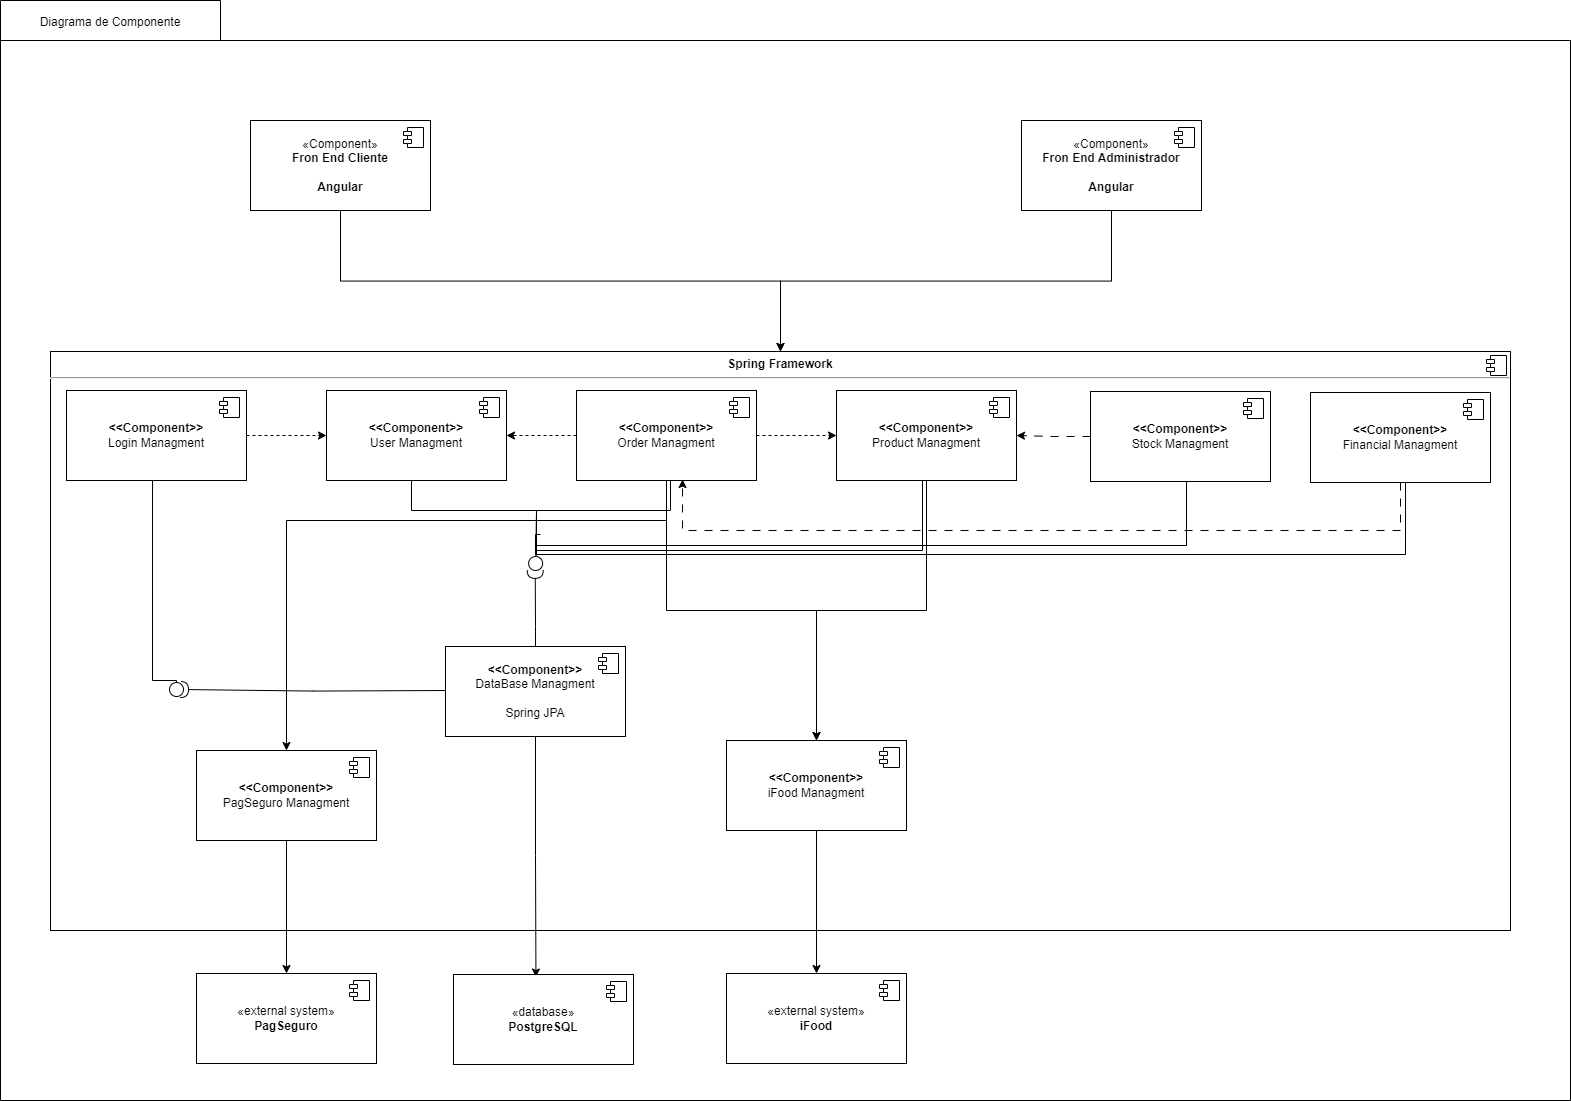
\includegraphics[width=1\textwidth]{diagrama_componentes.png}
    \caption{Diagrama de Componentes}
    \label{fig:Diagrama de Componentes}
  \end{figure}

  \href{https://github.com/soltein/TCC/blob/main/Diagramas/out/diagrama_componentes.png}{Imagem resolução maior}

  Podemos observar no diagrama de componentes que temos os seguintes componentes:

  \begin{itemize}
    \item frontend Cliente: Componente que representa o código feito utilizando framework Angular para interação do cliente com o sistema delivery.
    \item frontend Administrador: Componente que representa o código feito utilizando framework Angular para interação do atendente/administrador com o sistema delivery. Este será somente um front end e teremos os níveis de acesso.
    \item Login Managment: Componente que representa o código que será responsável pelo login do usuário.
    \item User Managment: Componente que representa o código que será responsável pelo controle dos usuários do sistema.
    \item Order Managment: Componente que representa o código que será responsável pelo controle das vendas do sistema.
    \item Product Managment: Componente que representa o código que será responsável pelo controle dos produtos do sistema.
    \item Stock Managment: Componente que representa o código que será responsável pelo controle de estoque do sistema.
    \item Financial Managment: Componente que representa o código que será responsável pelo controle das informações financeiras do sistema.
    \item Database Managment: Componente que representa o código que será responsável pelo controle de banco de dados.
    \item iFood Managment: Componente que representa o código que será responsável pelo controle da integração com o ifood do sistema.
    \item PagSeguro Managment: Componente que representa o código que será responsável pelo controle da integração com o pagseguro do sistema.
  \end{itemize}

\chapter{Vídeo Apresentação 1}
\href{https://youtu.be/eBemG0ewFlg}{Vídeo Apresentação 1}
\pgfmathsetmacro\nava{0}
\chapter{Avaliação Arquitetural ATAM}

A avaliação arquitetural ATAM (Architecture Tradeoff Analysis Method) tem como objetivo elicitar e refinar os requisitos de atributos de qualidade e 
as decisões de arquitetura no projeto de software.\cite{Mendes:2002}

\section{Análise das abordagens arquiteturais}
\vspace{0.5cm}

Abaixo listamos as abordagens arquiteturais, seus cenários, importância e complexidade(definidas em B - baixa, M - média e A - Alta).

\vspace{0.5cm}

\pgfmathtruncatemacro\nava{\nava + 1}
\subsection{Manutenabilidade}
Cenário \nava: A arquitetura deve considerar a facilidade de manutenção do sistema ao longo do tempo, buscando
criar uma estrutura que permita a evolução do sistema, isto pode ser atingido utilizando de padrões de projetos. 
Por exemplo na utilização do padrão MVC, separação das responsabilidades.

\vspace{0.5cm}
\noindent\textbf{\textit{Importância:}} \textit{A -} \textbf{\textit{Complexidade:}} \textit{A}
\vspace{0.5cm}

\pgfmathtruncatemacro\nava{\nava + 1}
\subsection{Usabilidade}
Cenário \nava: A arquitetura deve considerar a usabilidade do sistema, facilitando a utilização do mesmo por parte dos usuários,
além de permitir uma fácil integração de novos usuários ao sistema. Para isto deve se adotar padrões de interface, tanto em dispositivos
móveis como em telas maiores como monitores, utilizar de interfaces intuitivas e que o padrão seja mantido entre as telas do sistema.

\vspace{0.5cm}
\noindent\textbf{\textit{Importância:}} \textit{A -} \textbf{\textit{Complexidade:}} \textit{M}
\vspace{0.5cm}

\pgfmathtruncatemacro\nava{\nava + 1}
\subsection{Segurança}
Cenário \nava: A arquitetura deve ser pensada em tornar as informações protegidas e garantir acesso seguro ao sistema.
Um usuário não autorizado não deve conseguir acessar informações confidênciais do sistema. Para isso pdoe se adotar 
criptografia nas senhas e controle de autenticação e autorização no sistema.

\vspace{0.5cm}
\noindent\textbf{\textit{Importância:}} \textit{A -} \textbf{\textit{Complexidade:}} \textit{A}
\vspace{0.5cm}

\pgfmathtruncatemacro\nava{\nava + 1}
\subsection{Interoperabilidade}
Cenário \nava: A arquitetura deve considerar a capacidade do sistema em se comunicar com outros sistemas de software
em outras tecnologias, para isso deve-se adotar padrões de comunicação que são amplamente aceitos como RESTFUL, SOAP
e na utilização de formatos de dados amplamente utilizados como JSON e XML.

\vspace{0.5cm}
\noindent\textbf{\textit{Importância:}} \textit{A -} \textbf{\textit{Complexidade:}} \textit{M}
\vspace{0.5cm}

\pgfmathtruncatemacro\nava{\nava + 1}
\subsection{Desempenho}
Cenário \nava: A arquitetura deve considerar a capacidade do sistema em se manter estável e atingir requisitos de 
tempo de respostas quando de alta carga de trabalho, como horários de pico. Para isso a arquitetura deve ser pensada de modo 
a oferecer o dimensionamento de recursos, seja horizontal ou vertical e caches para informações estáticas.

\vspace{0.5cm}
\noindent\textbf{\textit{Importância:}} \textit{M -} \textbf{\textit{Complexidade:}} \textit{A}
\vspace{0.5cm}

\pgfmathsetmacro\cen{0}
\section{Cenários}
\vspace{0.5cm}

Abaixo listamos os cenários para serem efetuados testes na aplicação, os mesmos demonstram como serão satisfeitos os 
atributos de qualidade do software(requisitos não funcionais).

\pgfmathtruncatemacro\cen{\cen + 1}
\subsection{Cenário \cen} 
Manutenabilidade: Quando da necessidade de se atualizar um requisito de negócio do sistema, é necessário a modificação
em alguma camada do mesmo, portanto é fundamental o software ser desenvolvido em camadas e com baixo acoplamento 
entre as mesmas, permitindo assim uma fácil manutenção e evolução do software. O atendimento deste cenário atende o 
RNF-1 - Desenvolvimento em Camadas.

\pgfmathtruncatemacro\cen{\cen + 1}
\subsection{Cenário \cen} 
Usabilidade: Ao acessar o software de diferentes dispositivos o sistema deverá se adaptar ao tamanho das telas, além de 
ter um padrão visual entre telas e dispositivos de modo a facilitar o aprendizado do mesmo. O atendimento deste cenário 
atende o RNF-2 - Padrão de Interface.

\pgfmathtruncatemacro\cen{\cen + 1}
\subsection{Cenário \cen} 
Segurança: O sistema deverá criptografar dados sensivés do software, como a senha de acesso do usuário. O atendimento deste cenário 
atende o RNF-3 - Banco de dados.

\pgfmathtruncatemacro\cen{\cen + 1}
\subsection{Cenário \cen} 
Segurança: Ao tentar acessar um recurso privado sem estar logado o sistema deverá exibir uma mensagem de não autorizado. O atendimento deste cenário 
atende o RNF-4 - Autenticação/Autorização.

\pgfmathtruncatemacro\cen{\cen + 1}
\subsection{Cenário \cen} 
Interoperabilidade: Ao efetuar um pagamento através do software, o sistema deverá realizar uma comunicação com algum meio de pagamento para permitir a cobrança do cliente. O atendimento deste cenário 
atende o RNF-5 - Comunicação com sistema de pagamento.


\pgfmathtruncatemacro\cen{\cen + 1}
\subsection{Cenário \cen} 
Desempenho: Ao efetuar login no sistema, o mesmo deverá validar e permitir ou negar o acesso em até 5 segundos, permitindo assim uma
experiência fluida para o usuário. O atendimento deste cenário atende o RNF-6 - Acesso após Autenticação.

\pgfmathsetmacro\avcen{0}
\section{Evidências da Avaliação de Cenários}
\vspace{0.5cm}


\pgfmathtruncatemacro\avcen{\avcen + 1}
\subsection{Cenário \avcen} 
\noindent
\begin{tabular}{|>{\raggedright\arraybackslash}p{3cm}|>{\raggedright\arraybackslash}p{10cm}|}
    \hline
    \cellcolor[gray]{0.8}Atributo de Qualidade & Manutenabilidade \\
    \hline
    \cellcolor[gray]{0.8}Requisito de Qualidade & A arquitetura deve considerar a facilidade de manutenção do sistema ao longo do tempo, buscando criar uma estrutura que permita a evolução do sistema. \\
    \hline
    \multicolumn{2}{|l|}{\cellcolor[gray]{0.8}Preocupação:} \\
    \hline
    \multicolumn{2}{|p{13cm}|}{O sistema deverá ser feito utilizando padrão MVC, sendo assim desenvolvido em camadas de modo a facilitar a manutenabilidade do mesmo.} \\
    \hline
    \multicolumn{2}{|l|}{\cellcolor[gray]{0.8}Cenário(s):} \\
    \hline
    \multicolumn{2}{|p{13cm}|}{Cenário \avcen} \\
    \hline 
    \multicolumn{2}{|l|}{\cellcolor[gray]{0.8}Ambiente:} \\
    \hline        
    \multicolumn{2}{|p{13cm}|}{Operação normal} \\
    \hline     
    \multicolumn{2}{|l|}{\cellcolor[gray]{0.8}Estímulo:} \\
    \hline  
    \multicolumn{2}{|p{13cm}|}{Ao sofrer uma mudança de requisitos, como adição de novos campos.} \\    
    \hline     
    \multicolumn{2}{|l|}{\cellcolor[gray]{0.8}Mecanismo} \\
    \hline  
    \multicolumn{2}{|p{13cm}|}{Utilização de classes seguindo o modelo MVC e boas práticas de codificação de modo a separar as responsabilidades de cada classe} \\
    \hline 
    \multicolumn{2}{|l|}{\cellcolor[gray]{0.8}Medida de Resposta} \\
    \hline            
    \multicolumn{2}{|p{13cm}|}{Tempo gasto e facilidade para implementar mudanças de requisito} \\
    \hline 
    \multicolumn{2}{|l|}{\cellcolor[gray]{0.8}Considreação sobre a arquitetura:} \\
    \hline  
    \cellcolor[gray]{0.8}Riscos &  A adoção do padrão MVC pode resultar em uma arquitetura inicial mais complexa, exigindo uma correta implementação no decorrer do desenvolvimento.\\
    \hline           
    \cellcolor[gray]{0.8}Pontos de Sensibilidade &  Caso o sistema seja frequentemente alterado poderá vir a ser necessário uma revisão mais próxima e constante na estrutura da arquitetura para continuar garantindo a manutenabilidade.\\
    \hline           
    \cellcolor[gray]{0.8}Tradeoff &  No inicio do desenvolvimento poderá ocorrer um aumento na complexidade, o que será recompensado pela facilidade de manutenção a longo prazo.\\
    \hline         
\end{tabular}

\subsubsection{Evidência do Cenário \avcen} 

O desenvolvimento é no padrão arquitetural MVC, para isso utilizamos a separação das classes seguindo as regras do padrão, colocando
uma camada de controller para direcionar o fluxo, uma camada de modelo para representar as tabelas do banco, para isso utilizamos também o 
padrão repository e uma camada de serviço que contém as regras de negócio.

\begin{figure}[h]
   \centering
   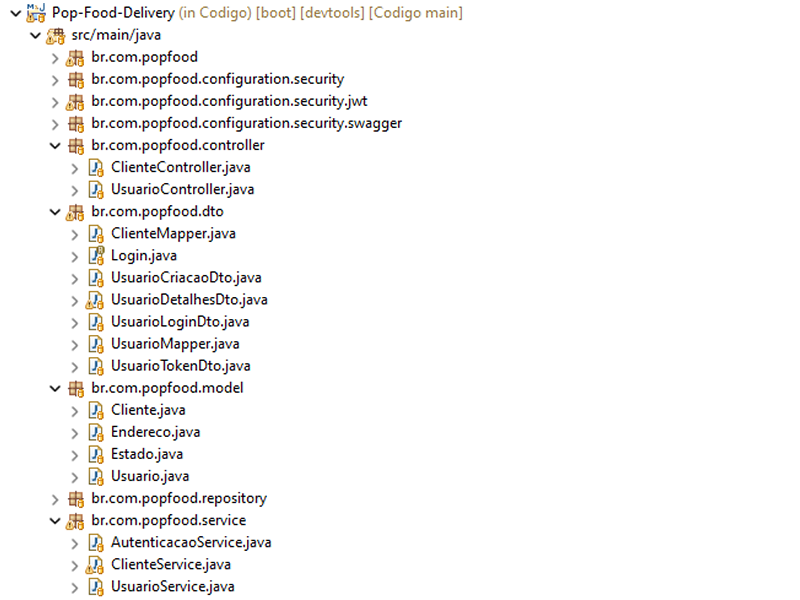
\includegraphics[width=1\textwidth]{padrao_mvc.png}
   \caption{Padrão MVC}
   \label{fig:Padrao MVC}
\end{figure}

\pgfmathtruncatemacro\avcen{\avcen + 1}
\subsection{Cenário \avcen} 
\noindent
\begin{tabular}{|>{\raggedright\arraybackslash}p{3cm}|>{\raggedright\arraybackslash}p{10cm}|}
    \hline
    \cellcolor[gray]{0.8}Atributo de Qualidade & Usabilidade \\
    \hline
    \cellcolor[gray]{0.8}Requisito de Qualidade & O software deve ter uma boa usabilidade mantendo o padrão e a adaptabilidade em diferentes telas. \\
    \hline
    \multicolumn{2}{|l|}{\cellcolor[gray]{0.8}Preocupação:} \\
    \hline
    \multicolumn{2}{|p{13cm}|}{Ao ser acessado de diferentes dispositivos o padrão deverá ser mantido e adaptado a resoluções diferentes.} \\
    \hline
    \multicolumn{2}{|l|}{\cellcolor[gray]{0.8}Cenário(s):} \\
    \hline
    \multicolumn{2}{|p{13cm}|}{Cenário \avcen} \\
    \hline 
    \multicolumn{2}{|l|}{\cellcolor[gray]{0.8}Ambiente:} \\
    \hline        
    \multicolumn{2}{|p{13cm}|}{Operação normal} \\
    \hline     
    \multicolumn{2}{|l|}{\cellcolor[gray]{0.8}Estímulo:} \\
    \hline  
    \multicolumn{2}{|p{13cm}|}{Ao acessar diferentes telas, o padrão deverá ser mantido e também adaptado a diferentes resoluções} \\    
    \hline     
    \multicolumn{2}{|l|}{\cellcolor[gray]{0.8}Mecanismo} \\
    \hline  
    \multicolumn{2}{|p{13cm}|}{Utilização de templates que permitam padronizar as telas e mantém uma boa usabilidade entre diferentes resoluções de tela.} \\
    \hline 
    \multicolumn{2}{|l|}{\cellcolor[gray]{0.8}Medida de Resposta} \\
    \hline            
    \multicolumn{2}{|p{13cm}|}{Tempo gasto de aprendizado na utilização do sistema} \\
    \hline 
    \multicolumn{2}{|l|}{\cellcolor[gray]{0.8}Considreação sobre a arquitetura:} \\
    \hline  
    \cellcolor[gray]{0.8}Riscos &  Caso tenha falhas na estrutura dos templates o sistema poderá ter inconsistências visuais, principalmente se utilizar de dispositivos que sejam muito fora do padrão ou mais antigos.\\
    \hline           
    \cellcolor[gray]{0.8}Pontos de Sensibilidade &  Dispositivos muito antigos ou com resoluções muito altas que fujam dos padrões existentes.\\
    \hline           
    \cellcolor[gray]{0.8}Tradeoff &  O desenvolvimento dos templates pode vir a exigir um esforço adicional durante o desenvolvimento, isso será compensado no futuro com a facilidade 
    de utilização do sistema e também para implementar novas funcionalidades, que seguirão um padrão já desenvolvido.\\
    \hline         
\end{tabular}

\subsubsection{Evidência do Cenário \avcen} 

No quesito de usabilidade optou-se por utilizar no front end o Angular Material, ele é baseado no Material Design e fornece
diversos componentes prontos e formas de se utilizar para se manter um padrão, tanto no quesito de aparência quanto na usabilidade do sistema.

Através da utilização do mesmo os componentes se ajustarão a diferentes resoluções e dispositivos, além de se manterem padronizados entre uma tela e outra de modo a facilitar o uso e aprendizado do sistema.

\begin{figure}[ht]
    \centering
    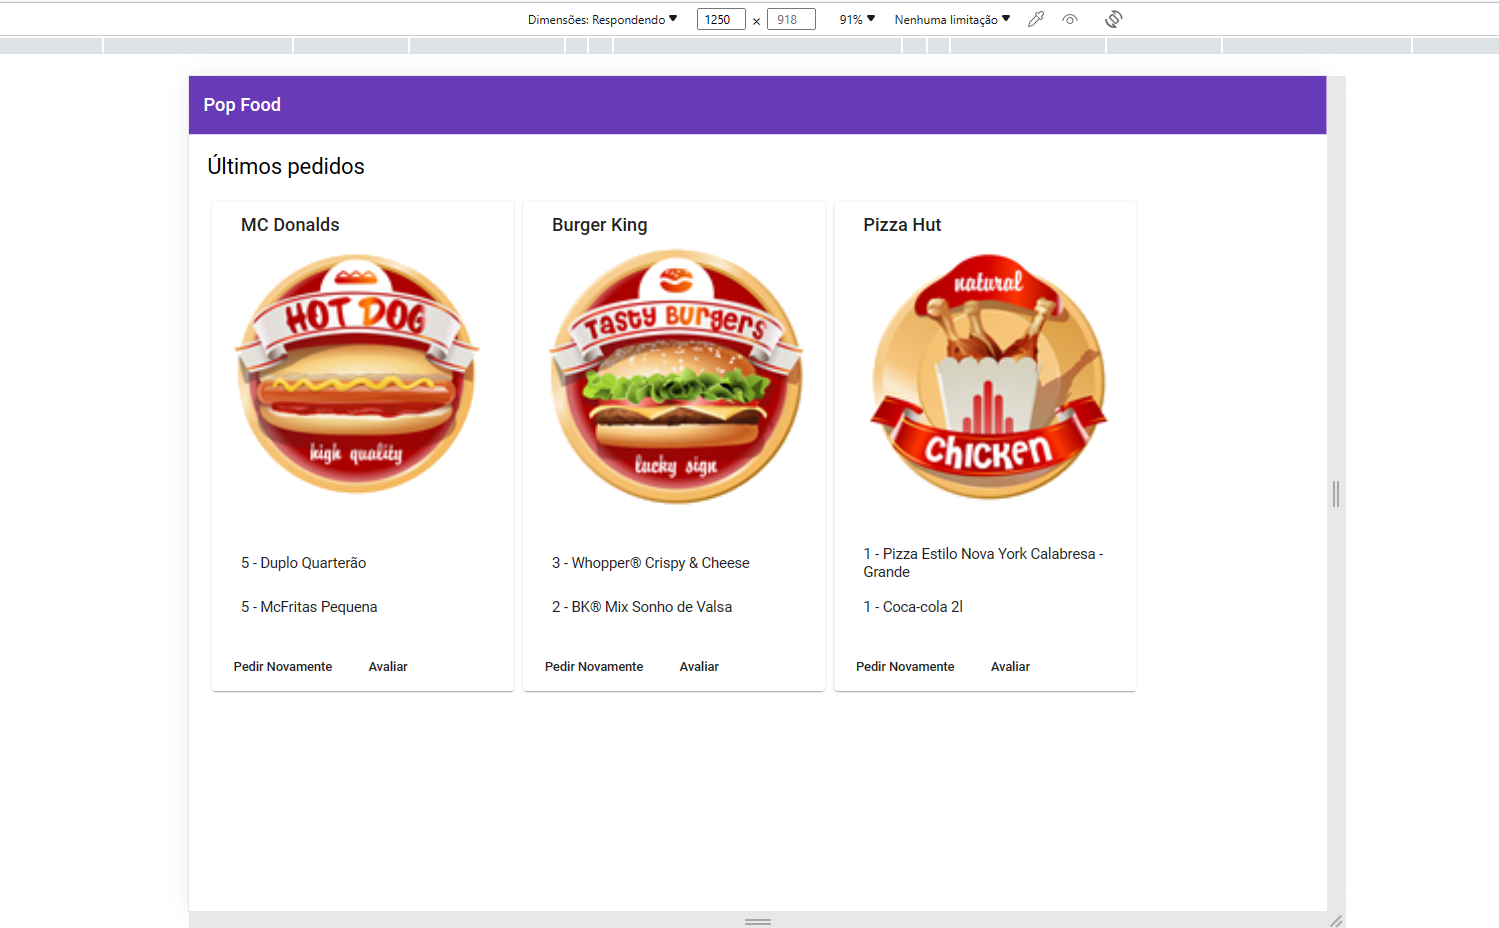
\includegraphics[width=1\textwidth]{front_end_navegador_material.png}
    \caption{Utilização do Angular Material - Visualização Navegador}
    \label{fig:Angular Material}
 \end{figure}

 \begin{figure}[ht]
    \centering
    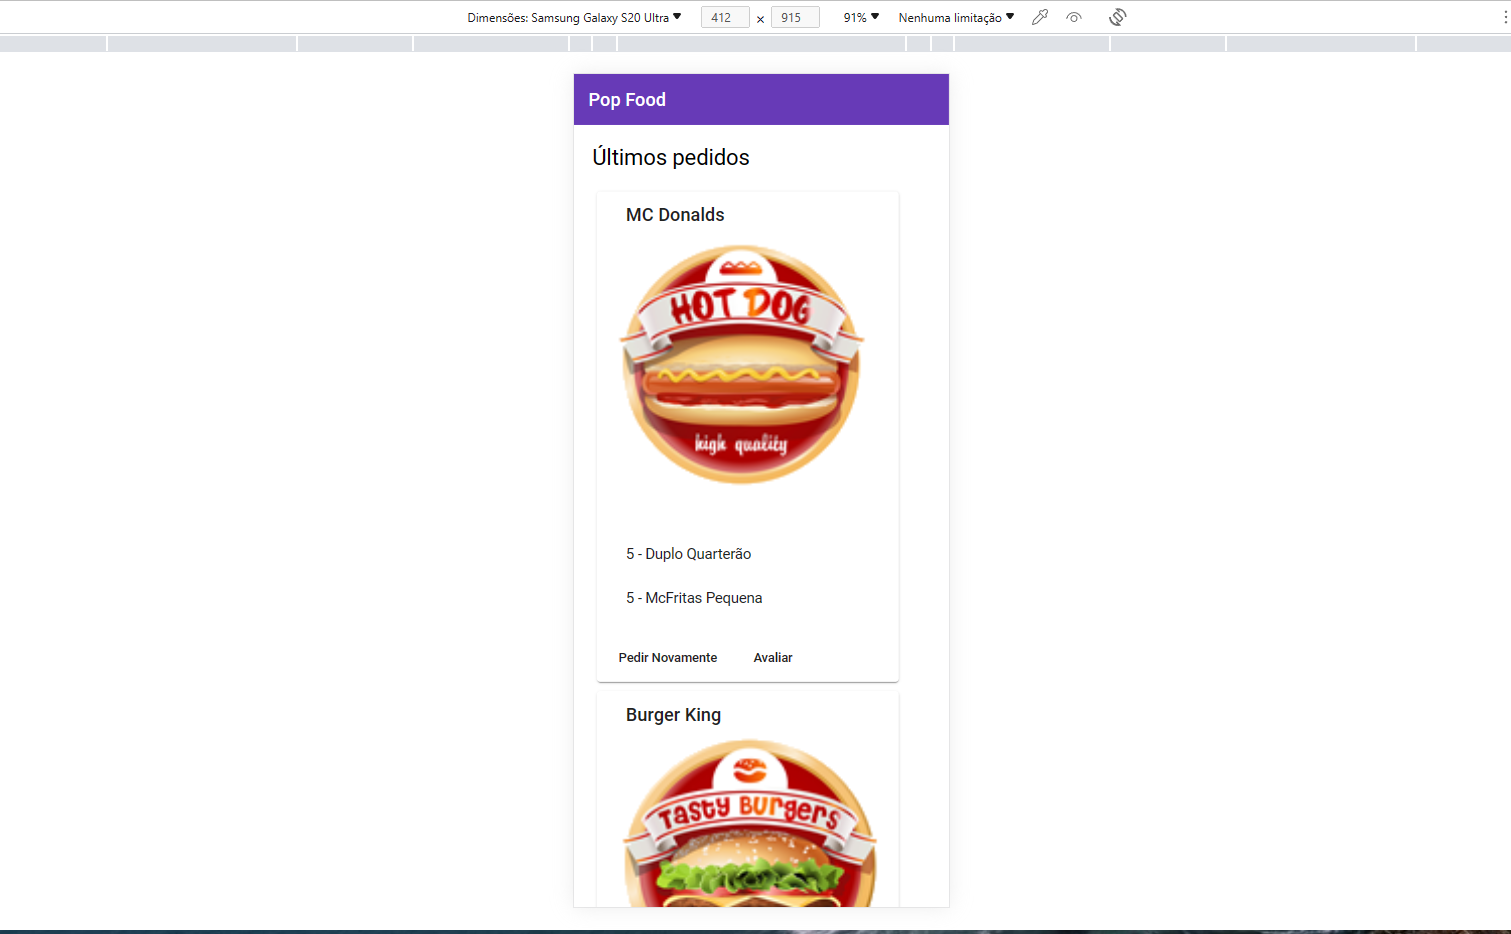
\includegraphics[width=1\textwidth]{front_end_celular_material.png}
    \caption{Utilização do Angular Material - Visualização Celular}
    \label{fig:Angular Material Celular}
 \end{figure}



\pgfmathtruncatemacro\avcen{\avcen + 1}
\subsection{Cenário \avcen} 
\noindent
\begin{tabular}{|>{\raggedright\arraybackslash}p{3cm}|>{\raggedright\arraybackslash}p{10cm}|}
    \hline
    \cellcolor[gray]{0.8}Atributo de Qualidade & Segurança \\
    \hline
    \cellcolor[gray]{0.8}Requisito de Qualidade &  O sistema deverá criptografar dados sensíveis do software, como a senha de acesso do usuário.\\
    \hline
    \multicolumn{2}{|l|}{\cellcolor[gray]{0.8}Preocupação:} \\
    \hline
    \multicolumn{2}{|p{13cm}|}{Proteger informações sensíveis por meio de criptografia para evitar acesso não autorizado aos dados.} \\
    \hline
    \multicolumn{2}{|l|}{\cellcolor[gray]{0.8}Cenário(s):} \\
    \hline
    \multicolumn{2}{|p{13cm}|}{Cenário \avcen} \\
    \hline 
    \multicolumn{2}{|l|}{\cellcolor[gray]{0.8}Ambiente:} \\
    \hline        
    \multicolumn{2}{|p{13cm}|}{Operação normal} \\
    \hline     
    \multicolumn{2}{|l|}{\cellcolor[gray]{0.8}Estímulo:} \\
    \hline  
    \multicolumn{2}{|p{13cm}|}{Tentativa não autorizada de acesso a senha do usuário} \\    
    \hline     
    \multicolumn{2}{|l|}{\cellcolor[gray]{0.8}Mecanismo} \\
    \hline  
    \multicolumn{2}{|p{13cm}|}{Utilização de algoritmos de criptografia para proteger a senha do usuário.} \\
    \hline 
    \multicolumn{2}{|l|}{\cellcolor[gray]{0.8}Medida de Resposta} \\
    \hline            
    \multicolumn{2}{|p{13cm}|}{Dificultar descobrir a senha do usuário.} \\
    \hline 
    \multicolumn{2}{|l|}{\cellcolor[gray]{0.8}Considreação sobre a arquitetura:} \\
    \hline  
    \cellcolor[gray]{0.8}Riscos & Não basta somente criptografar a senha, pois poderão pegar a criptografia e tentar comparar com senhas comuns e então encontrar a senha do usuário, portanto, torna-se necessário acrescentar alguma informação a senha, como um salt(técnica que consiste em adicionar alguma informação secreta a senha, e quando o usuário digitar a senha o sistema acrescenta a informação antes da comparação) que combinado a senha gere a criptografia. \\
    \hline           
    \cellcolor[gray]{0.8}Pontos de Sensibilidade & NA \\
    \hline           
    \cellcolor[gray]{0.8}Tradeoff & NA \\
    \hline         
\end{tabular}

\subsubsection{Evidência do Cenário \avcen} 

No quesito de segurança optou por criptografar os dados sensivéis, a principio foi identificado a senha como uma informação sensível, sendo necessário 
avaliar as demais informações para definir o que deve ser criptografado.

\begin{figure}[ht]
    \centering
    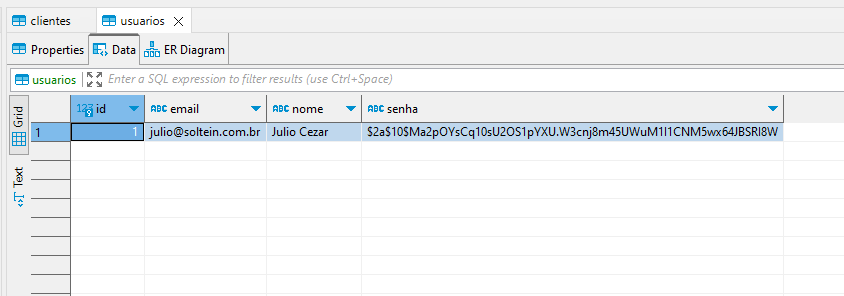
\includegraphics[width=1\textwidth]{senha_criptografada.png}
    \caption{Segurança criptografia senha}
    \label{fig:Segurança criptografia senha}
 \end{figure}

\pgfmathtruncatemacro\avcen{\avcen + 1}
\subsection{Cenário \avcen} 
\noindent
\begin{tabular}{|>{\raggedright\arraybackslash}p{3cm}|>{\raggedright\arraybackslash}p{10cm}|}
    \hline
    \cellcolor[gray]{0.8}Atributo de Qualidade & Segurança \\
    \hline
    \cellcolor[gray]{0.8}Requisito de Qualidade &  Ao tentar acessar um recurso privado sem estar logado, o sistema deverá exibir uma mensagem de não autorizado.\\
    \hline
    \multicolumn{2}{|l|}{\cellcolor[gray]{0.8}Preocupação:} \\
    \hline
    \multicolumn{2}{|p{13cm}|}{Garantir que somente usuários autorizados tenham acesso aos recursos privados.} \\
    \hline
    \multicolumn{2}{|l|}{\cellcolor[gray]{0.8}Cenário(s):} \\
    \hline
    \multicolumn{2}{|p{13cm}|}{Cenário \avcen} \\
    \hline 
    \multicolumn{2}{|l|}{\cellcolor[gray]{0.8}Ambiente:} \\
    \hline        
    \multicolumn{2}{|p{13cm}|}{Operação normal} \\
    \hline     
    \multicolumn{2}{|l|}{\cellcolor[gray]{0.8}Estímulo:} \\
    \hline  
    \multicolumn{2}{|p{13cm}|}{Tentativa de acesso a recurso privado sem estar logado} \\    
    \hline     
    \multicolumn{2}{|l|}{\cellcolor[gray]{0.8}Mecanismo} \\
    \hline  
    \multicolumn{2}{|p{13cm}|}{Implementação de um controle de autenticação e autorização que verifica se o usuário está logado e possui as permissões necessárias para acessar o recurso.} \\
    \hline 
    \multicolumn{2}{|l|}{\cellcolor[gray]{0.8}Medida de Resposta} \\
    \hline            
    \multicolumn{2}{|p{13cm}|}{Não autorizar acesso a recursos privados do software.} \\
    \hline 
    \multicolumn{2}{|l|}{\cellcolor[gray]{0.8}Consideração sobre a arquitetura:} \\
    \hline  
    \cellcolor[gray]{0.8}Riscos &  Implementação de um controle de autenticação e autorização que verifica se o usuário está logado e possui as permissões necessárias para acessar o recurso. \\
    \hline           
    \cellcolor[gray]{0.8}Pontos de Sensibilidade & NA \\
    \hline           
    \cellcolor[gray]{0.8}Tradeoff & NA \\
    \hline         
\end{tabular}

\subsubsection{Evidência do Cenário \avcen} 

Neste quesito foi desenvolvido um módulo de autenticação baseado em JWT(JSON Web Token), pois ele é utilizado amplamente 
em autenticação de sistemas, o back end ao receber os dados de acesso gera um token temporário que permite ao usuário acessar 
áreas privadas do sistema.

\begin{figure}[ht]
    \centering
    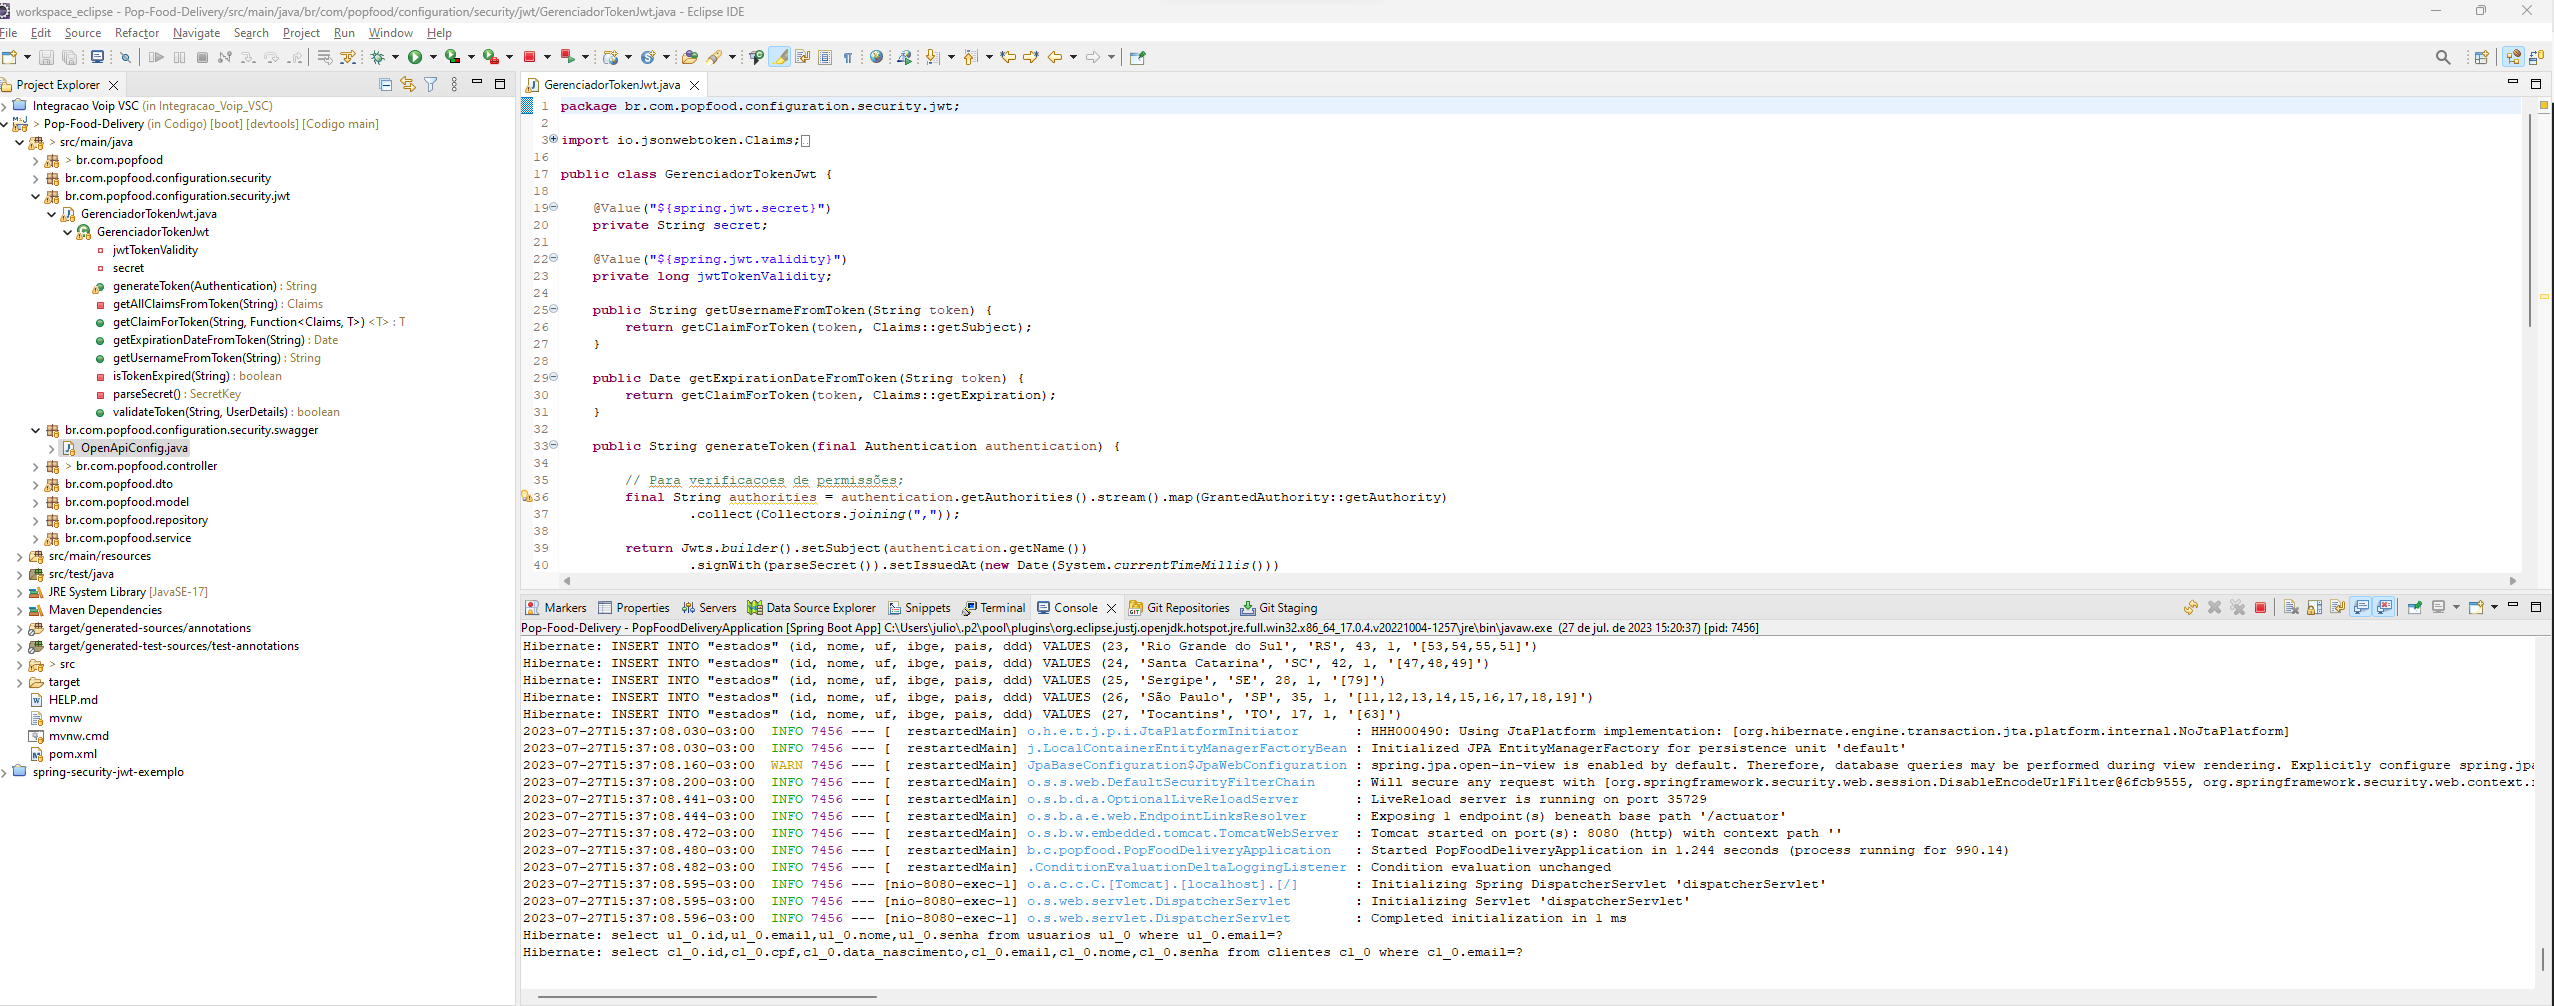
\includegraphics[width=1\textwidth]{codigo_fonte_jwt.png}
    \caption{Parte do código responsável pelo JWT.}
    \label{fig:Parte do código responsável pelo JWT.}
 \end{figure}

\begin{figure}[ht]
    \centering
    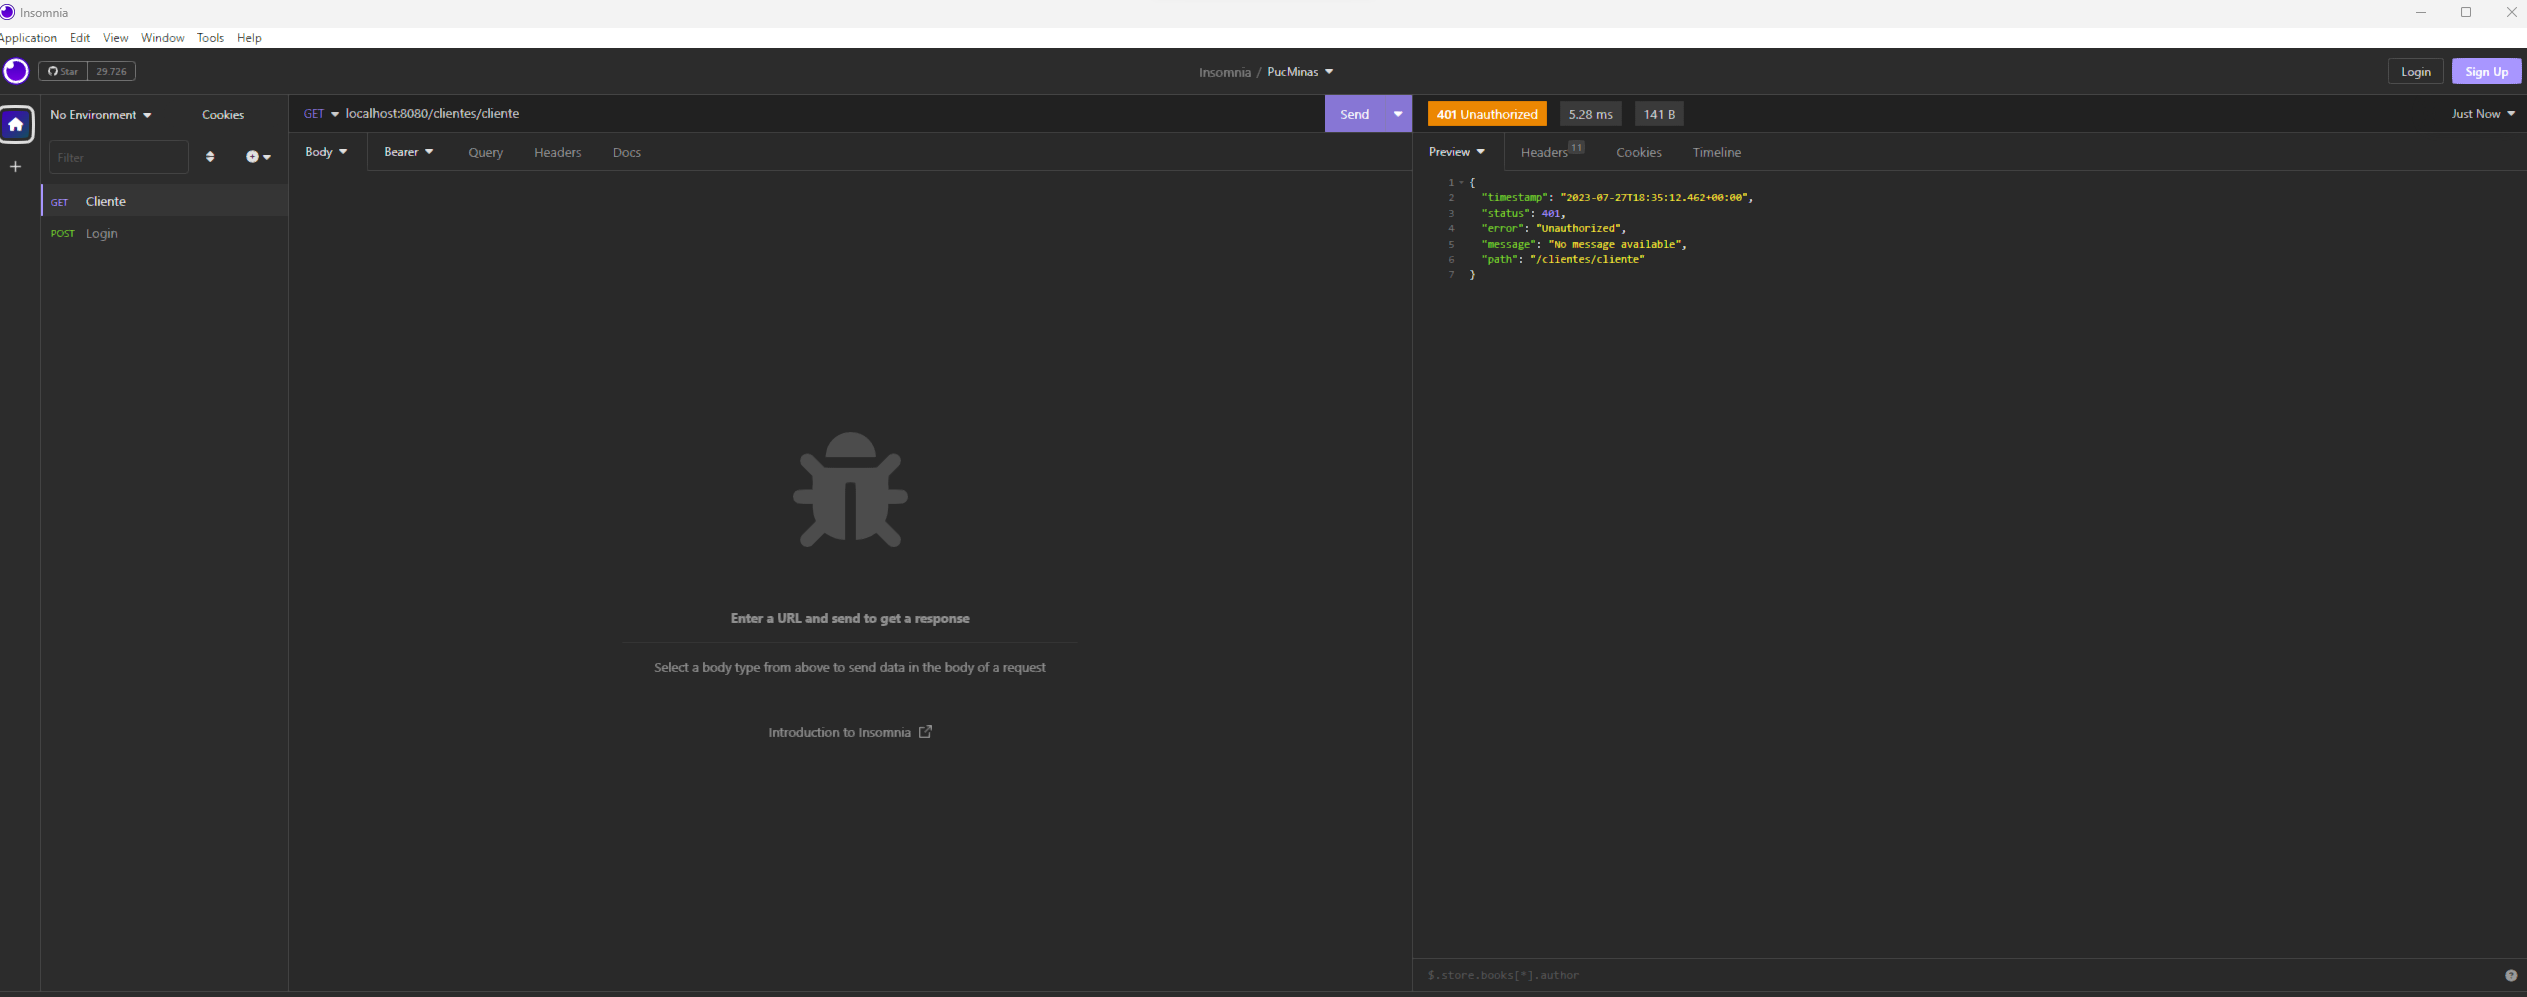
\includegraphics[width=1\textwidth]{acesso_sem_token.png}
    \caption{Tentativa de acesso sem estar logado.}
    \label{fig:Tentativa de acesso sem estar logado.}
 \end{figure}

 \begin{figure}[ht]
    \centering
    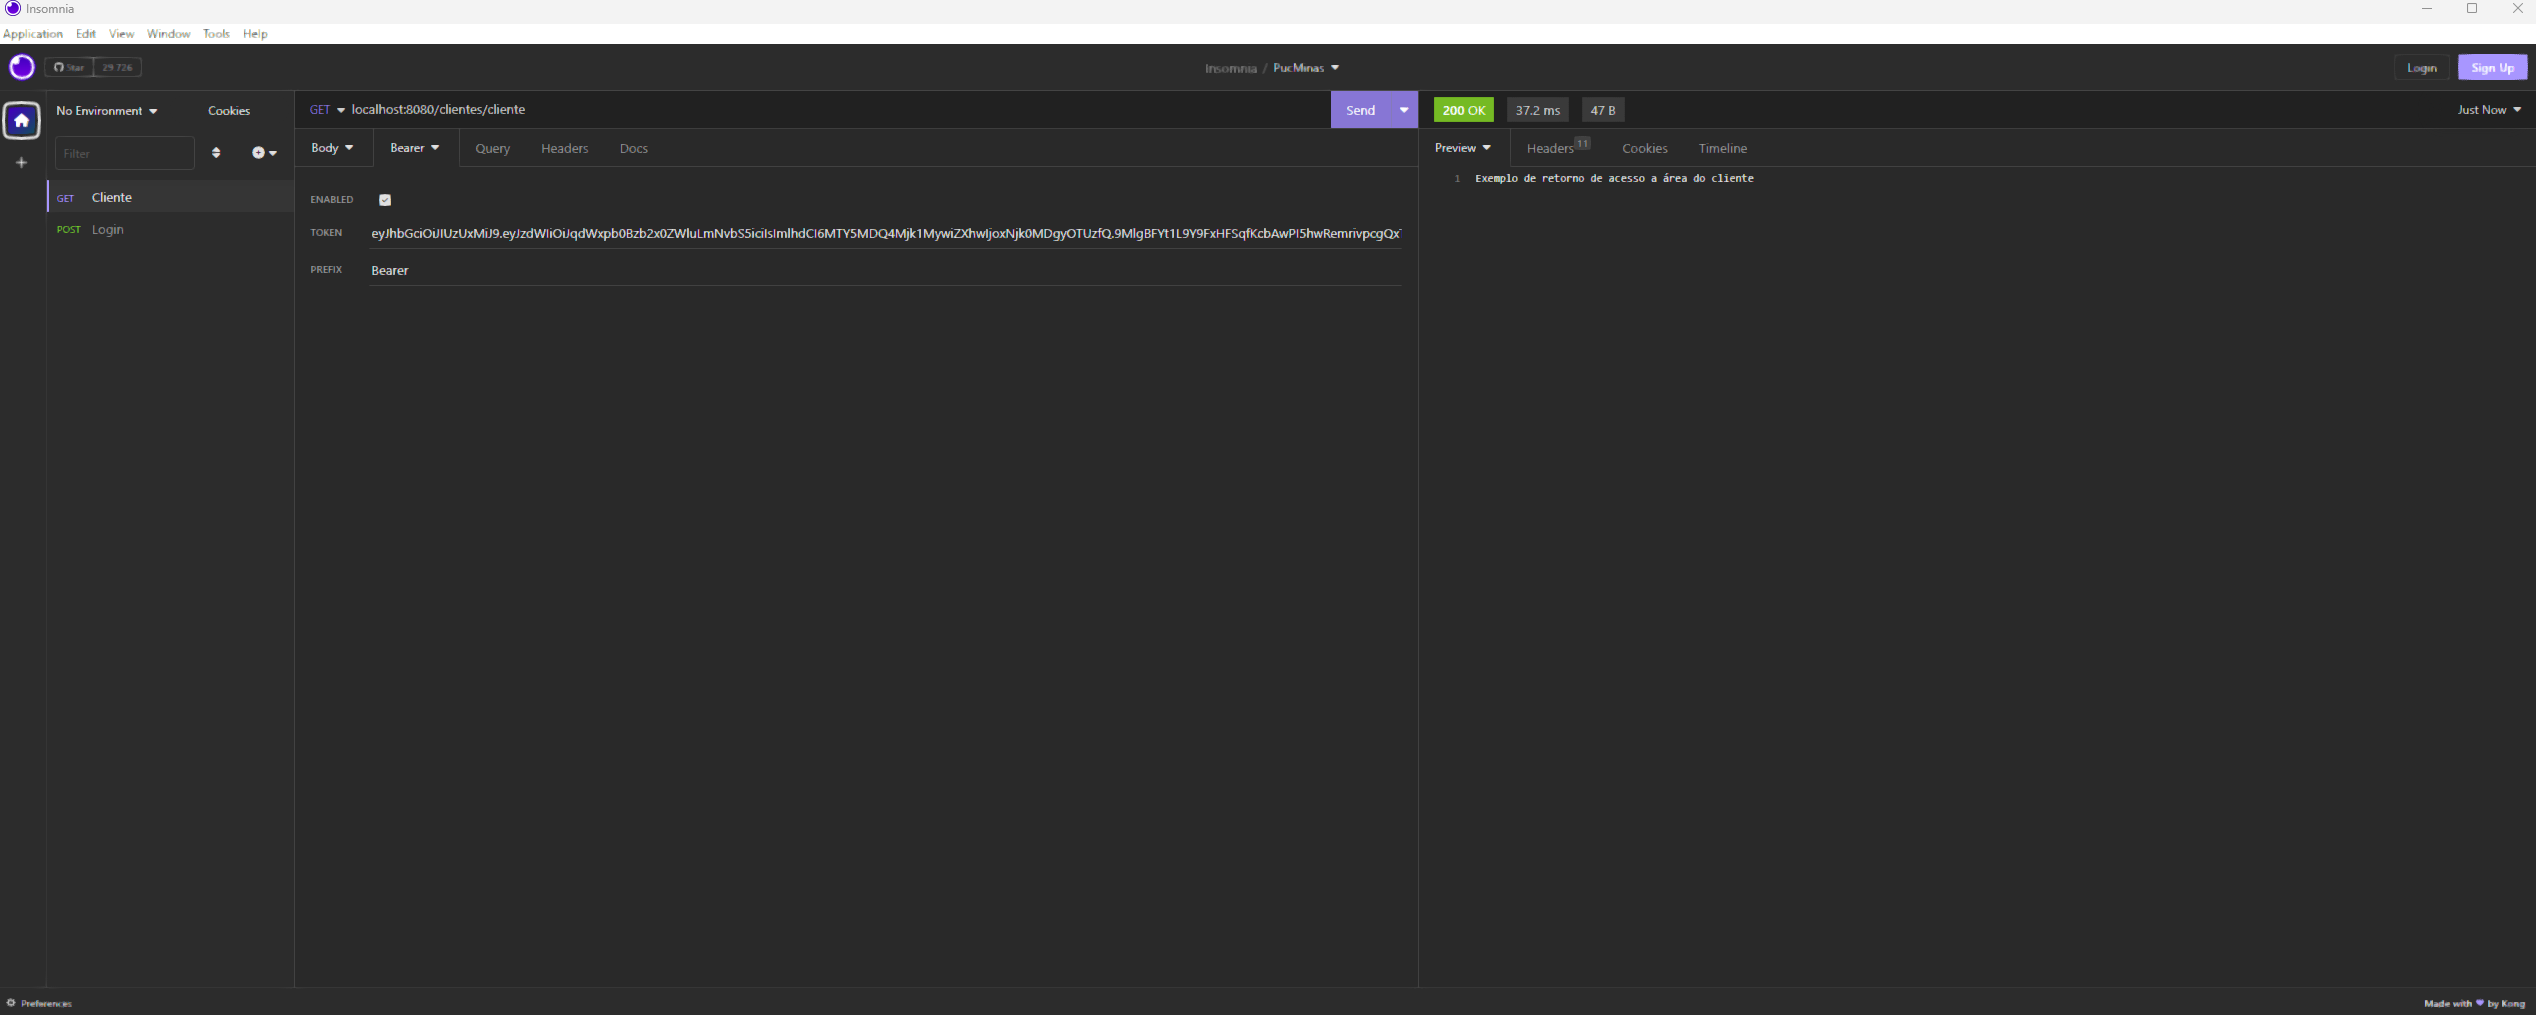
\includegraphics[width=1\textwidth]{acesso_com_token.png}
    \caption{Tentativa de acesso logado ao sistema.}
    \label{fig:Tentativa de acesso logao ao sistema.}
 \end{figure}



 \pgfmathtruncatemacro\avcen{\avcen + 1}
 \subsection{Cenário \avcen} 
 \noindent
 \begin{tabular}{|>{\raggedright\arraybackslash}p{3cm}|>{\raggedright\arraybackslash}p{10cm}|}
     \hline
     \cellcolor[gray]{0.8}Atributo de Qualidade & Interoperabilidade \\
     \hline
     \cellcolor[gray]{0.8}Requisito de Qualidade &  O sistema deve considerar a capacidade de se comunicar com outros sistemas de software em outras tecnologias, adotando padrões de comunicação amplamente aceitos, como RESTful, utilizando formatos de dados amplamente utilizados como JSON.\\
     \hline
     \multicolumn{2}{|l|}{\cellcolor[gray]{0.8}Preocupação:} \\
     \hline
     \multicolumn{2}{|p{13cm}|}{Garantir que o sistema possa integrar-se com outros sistemas de software, utilizando padrões amplamente adotados no mercado.} \\
     \hline
     \multicolumn{2}{|l|}{\cellcolor[gray]{0.8}Cenário(s):} \\
     \hline
     \multicolumn{2}{|p{13cm}|}{Cenário \avcen} \\
     \hline 
     \multicolumn{2}{|l|}{\cellcolor[gray]{0.8}Ambiente:} \\
     \hline        
     \multicolumn{2}{|p{13cm}|}{Operação normal} \\
     \hline     
     \multicolumn{2}{|l|}{\cellcolor[gray]{0.8}Estímulo:} \\
     \hline  
     \multicolumn{2}{|p{13cm}|}{Necessidade do cliente efetuar um pagamento online do pedido.} \\    
     \hline     
     \multicolumn{2}{|l|}{\cellcolor[gray]{0.8}Mecanismo} \\
     \hline  
     \multicolumn{2}{|p{13cm}|}{Utilização de protocolos de comunicação amplamente aceitos, como RESTful, para integrar com o meio de pagamento externo.} \\
     \hline 
     \multicolumn{2}{|l|}{\cellcolor[gray]{0.8}Medida de Resposta} \\
     \hline            
     \multicolumn{2}{|p{13cm}|}{Sucesso na comunicação e integração com o meio de pagamento externo, evidenciado pela realização bem-sucedida de transações e processamentos de pagamento.} \\
     \hline 
     \multicolumn{2}{|l|}{\cellcolor[gray]{0.8}Consideração sobre a arquitetura:} \\
     \hline  
     \cellcolor[gray]{0.8}Riscos & Os sistemas podem estar vulneráveis a ameaças de segurança, levando ao comprometimento de dados e roubos de informações sensíveis, principalmente por se tratar
     de dados de pagamento. Portanto é necessário verificar as diversas possibilidades, como a tela em que o usuário digita as informações de cartão já ser uma tela da operadora, dessa forma não teremos a responsabilidade sobre as informações. \\
     \hline           
     \cellcolor[gray]{0.8}Pontos de Sensibilidade & Um dos principais pontos de sensibilidade é o armazenamento das informações de cartões, deve-se decidir se essas informações ficarão armazenadas ou se encontrará uma operadora em que os dados sejam digitados em seu sistema.
     Caso opte por armazenar, é necessário uma evolução maior da arquitetura pois ai iremos tratar de implementações como certificação PCI o que aumenta a complexidade do sistema e infra-estrutura. \\
     \hline           
     \cellcolor[gray]{0.8}Tradeoff & É importante equilibrar a segurança com os desejos de funcionalidades do sistema, é de grande desejo ter a opção de pagamento online, mas devemos ter uma visão 
     sobre a segurança desta funcionalidade e o riscos e prejuízos em casos de falha. Portanto é necessário encontrar um meio termo como informado anteriormente, uma plataforma que já tenha esse nível de segurança garantido e processamos somente 
     enviar dados não sensíveis e esta plataforma cuidar das informações mais sensíveis como dados de cartão. \\
     \hline         
 \end{tabular}
 
 \subsubsection{Evidência do Cenário \avcen} 

 Foi desenvolvido um POC para simular a integração com a CIELO, utilizamos da documentação deles e desenvolvemos um exemplo fictício com o objetivo de testar a 
 tecnologia utilizada, no caso RestTemplet do Spring. 

 Neste POC criamos uma chamada ao end point da CIELO passando as informações via JSON e obtemos o retorno de sucesso da geração do pedido de compra nos sistemas deles.


 \begin{figure}[ht]
    \centering
    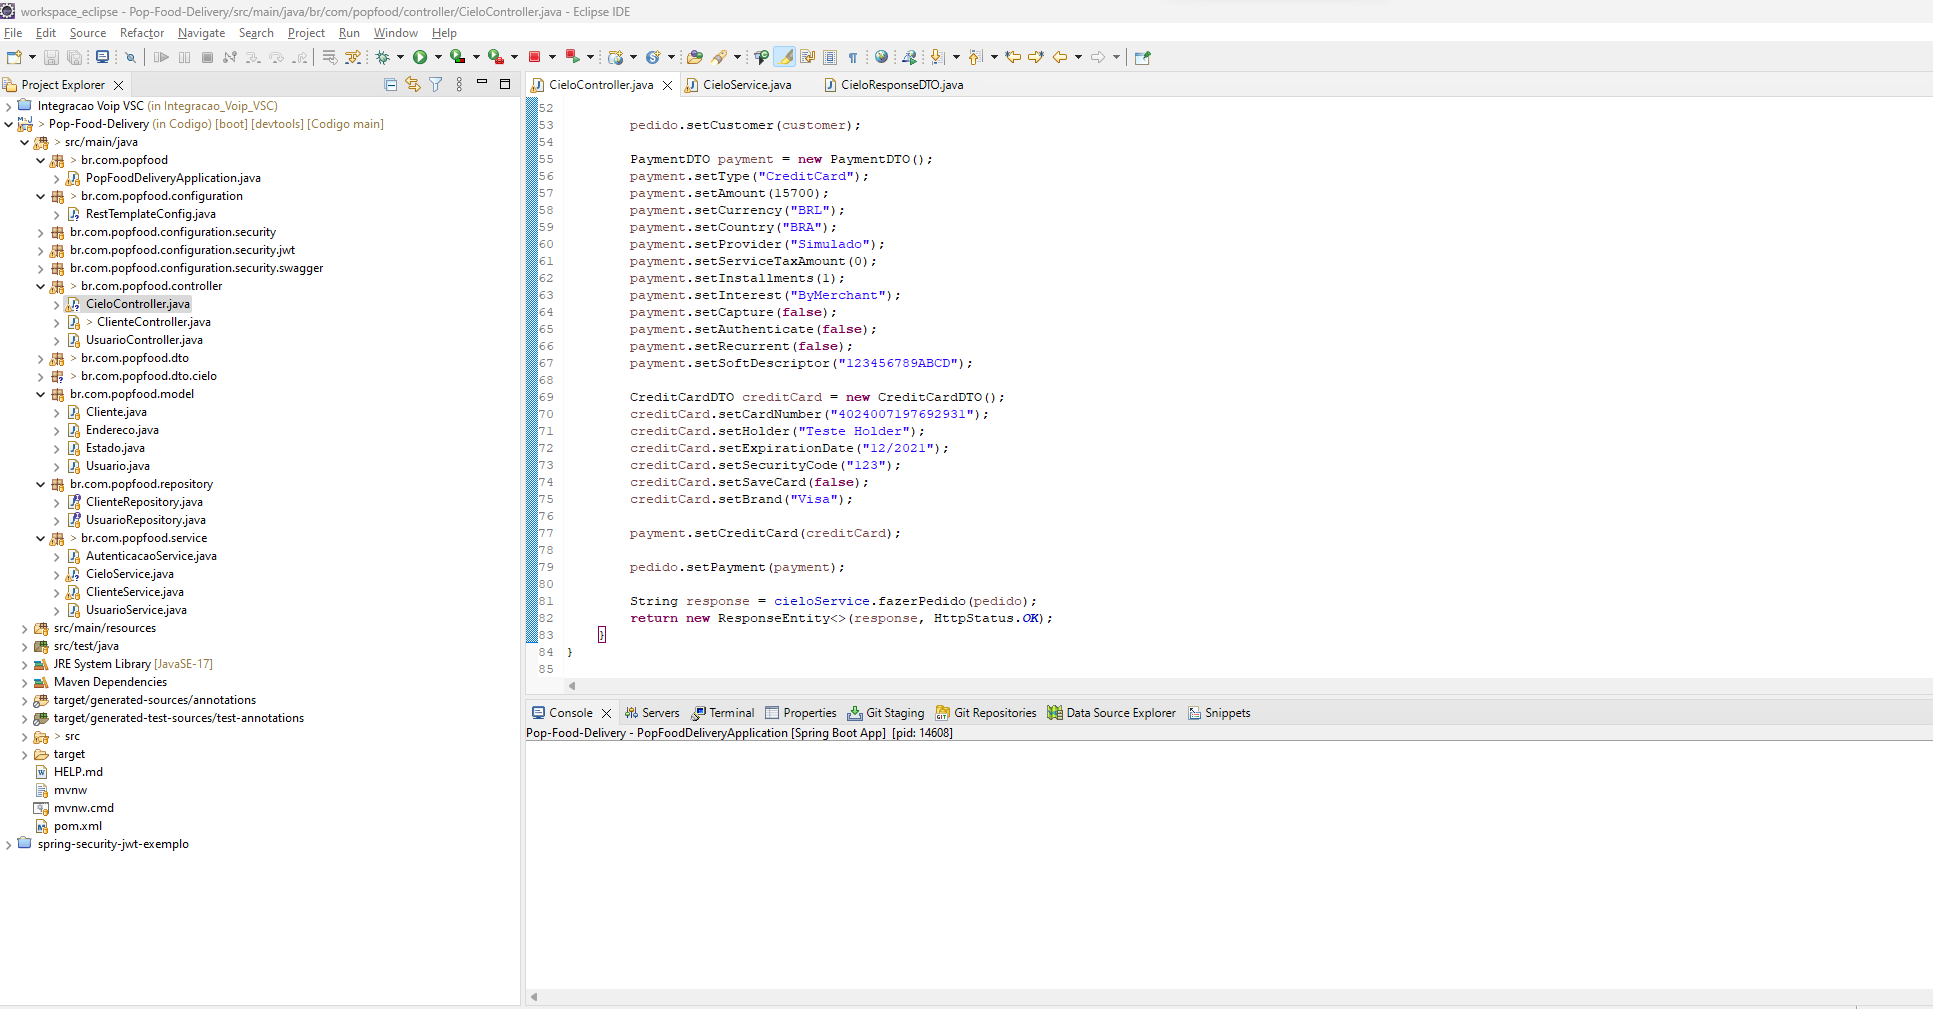
\includegraphics[width=1\textwidth]{interoperabilidade_cielo_controller.png}
    \caption{Código fonte controller POC - CIELO.}
    \label{fig:Código fonte controller POC - CIELO.}
 \end{figure}

 \begin{figure}[ht]
    \centering
    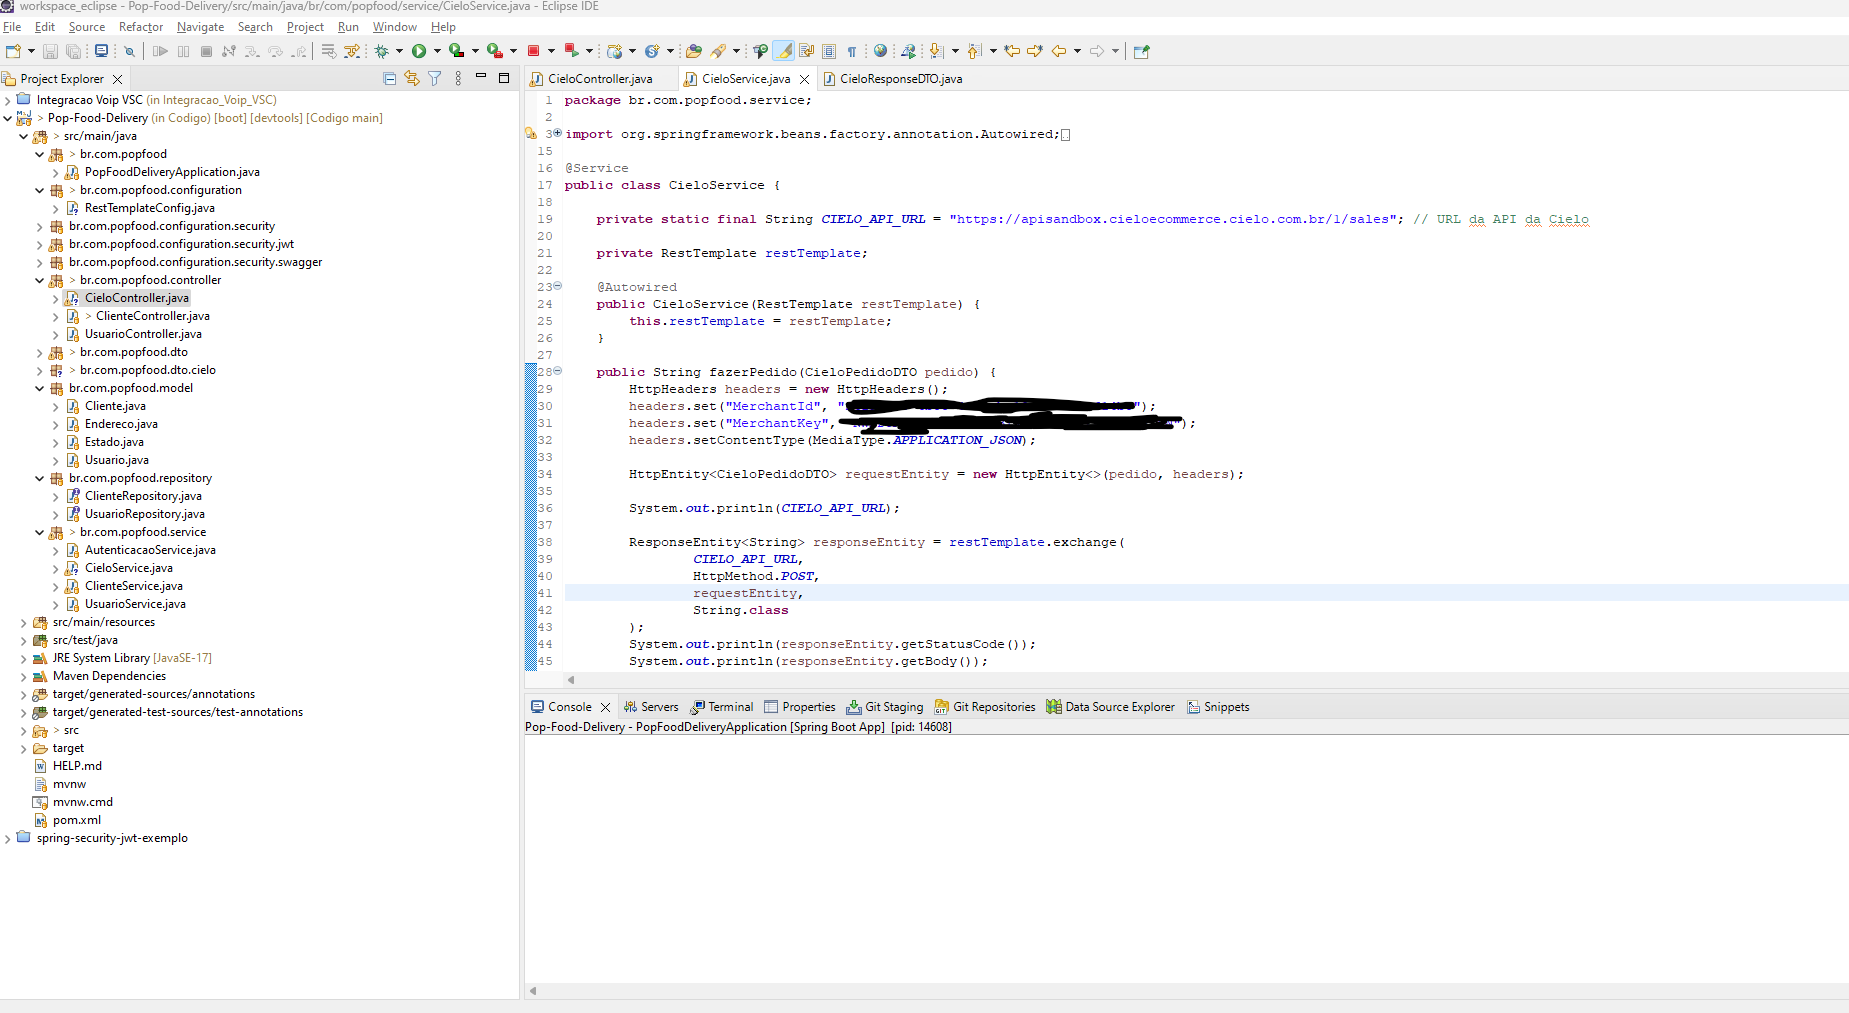
\includegraphics[width=1\textwidth]{interoperabilidade_cielo_service.png}
    \caption{Código fonte service POC - CIELO.}
    \label{fig:Código fonte service POC - CIELO.}
 \end{figure}

 \begin{figure}[ht]
    \centering
    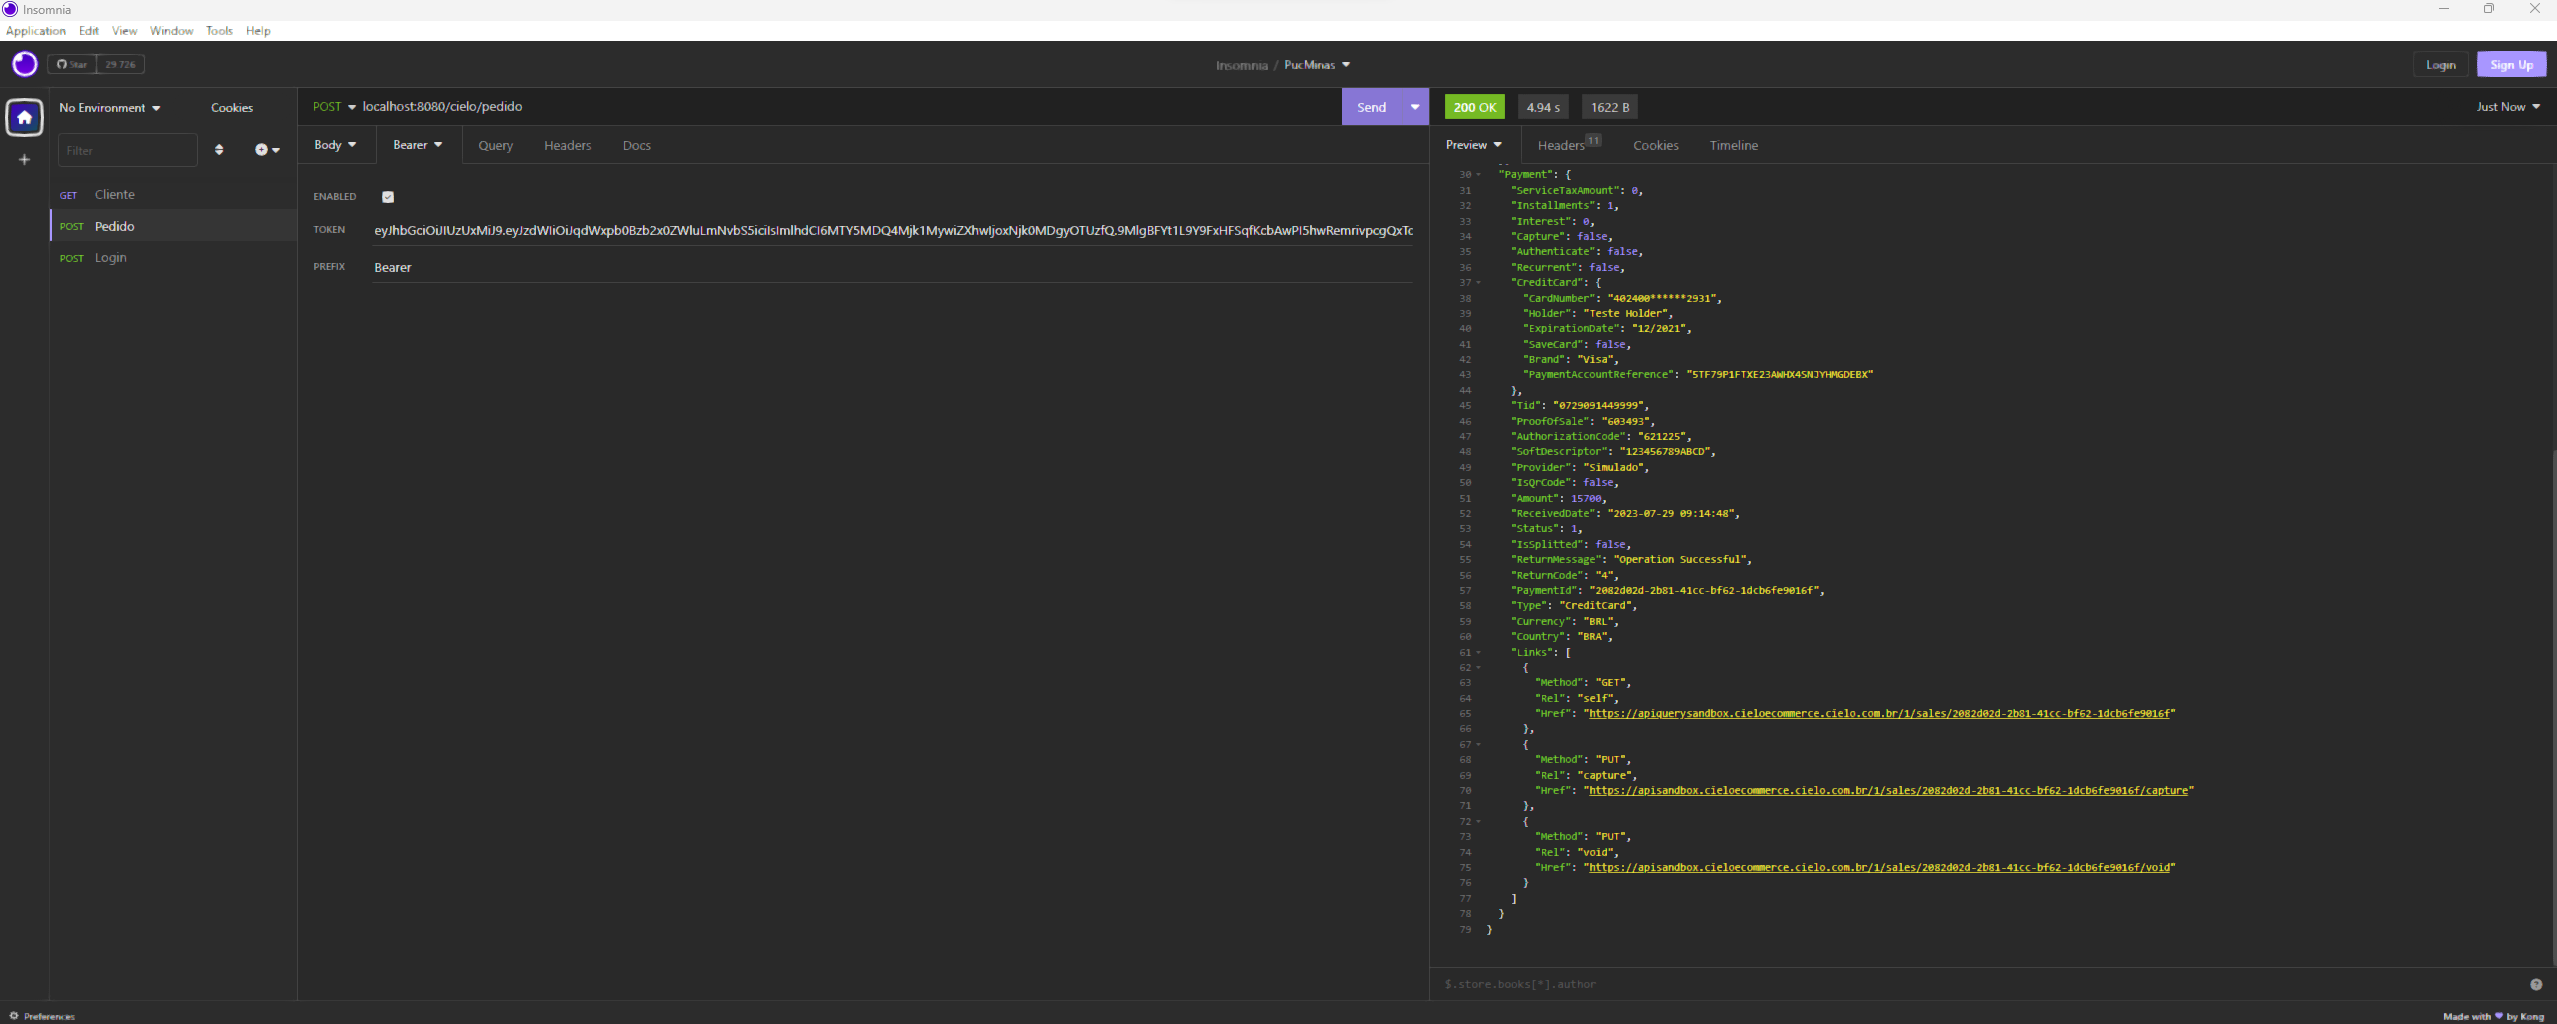
\includegraphics[width=1\textwidth]{interoperabilidade_retorno_insominia.png}
    \caption{Teste de execução com INSOMINIA POC - CIELO.}
    \label{fig:Teste de execução com INSOMINIA POC - CIELO.}
 \end{figure}



 \pgfmathtruncatemacro\avcen{\avcen + 1}
 \subsection{Cenário \avcen} 
 \noindent
 \begin{tabular}{|>{\raggedright\arraybackslash}p{3cm}|>{\raggedright\arraybackslash}p{10cm}|}
     \hline
     \cellcolor[gray]{0.8}Atributo de Qualidade & Desempenho \\
     \hline
     \cellcolor[gray]{0.8}Requisito de Qualidade &   O sistema deve ser capaz de exibir sua tela inicial após a inserção dos dados de acesso em menos de 5 segundos.\\
     \hline
     \multicolumn{2}{|l|}{\cellcolor[gray]{0.8}Preocupação:} \\
     \hline
     \multicolumn{2}{|p{13cm}|}{Garantir que o sistema ofereça uma experiência fluida para o usuário ao efetuar o login, proporcionando tempo de resposta rápido e eficiente.} \\
     \hline
     \multicolumn{2}{|l|}{\cellcolor[gray]{0.8}Cenário(s):} \\
     \hline
     \multicolumn{2}{|p{13cm}|}{Cenário \avcen} \\
     \hline 
     \multicolumn{2}{|l|}{\cellcolor[gray]{0.8}Ambiente:} \\
     \hline        
     \multicolumn{2}{|p{13cm}|}{Operação normal} \\
     \hline     
     \multicolumn{2}{|l|}{\cellcolor[gray]{0.8}Estímulo:} \\
     \hline  
     \multicolumn{2}{|p{13cm}|}{Efetuar login no sistema.} \\    
     \hline     
     \multicolumn{2}{|l|}{\cellcolor[gray]{0.8}Mecanismo} \\
     \hline  
     \multicolumn{2}{|p{13cm}|}{Implementação de estratégia de autenticação otimizada baseada em usuário e senha. Utilização de JTW para geração de token a ser validado nas rotas privadas da aplicação.} \\
     \hline 
     \multicolumn{2}{|l|}{\cellcolor[gray]{0.8}Medida de Resposta} \\
     \hline            
     \multicolumn{2}{|p{13cm}|}{Tempo de resposta na geração do TOKEN de acesso as demais telas do sistema.} \\
     \hline 
     \multicolumn{2}{|l|}{\cellcolor[gray]{0.8}Consideração sobre a arquitetura:} \\
     \hline  
     \cellcolor[gray]{0.8}Riscos & Uma sobrecarga do servidor em caso de grande número de acessos simultâneos poderá acarretar em degradação do desempenho do sistema como um todo. \\
     \hline           
     \cellcolor[gray]{0.8}Pontos de Sensibilidade &  NA\\
     \hline           
     \cellcolor[gray]{0.8}Tradeoff & NA \\
     \hline         
 \end{tabular}
 
 \subsubsection{Evidência do Cenário \avcen} 

 Foi efetuada a simulação de acesso ao sistema utilizando o INSOMINIA, nele foi verificado que o sistema em operação normal 
 o acesso é muito rápido, ficando em 82.4 ms. É claro que no uso diário do sistema deverá ser acompanhado o crescimento do mesmo e a 
 quantidade de usuários simultâneos, e caso necessário a infra-estrutura deverá crescer vertical e horizontalmente para atender a demanda.

 \begin{figure}[ht]
    \centering
    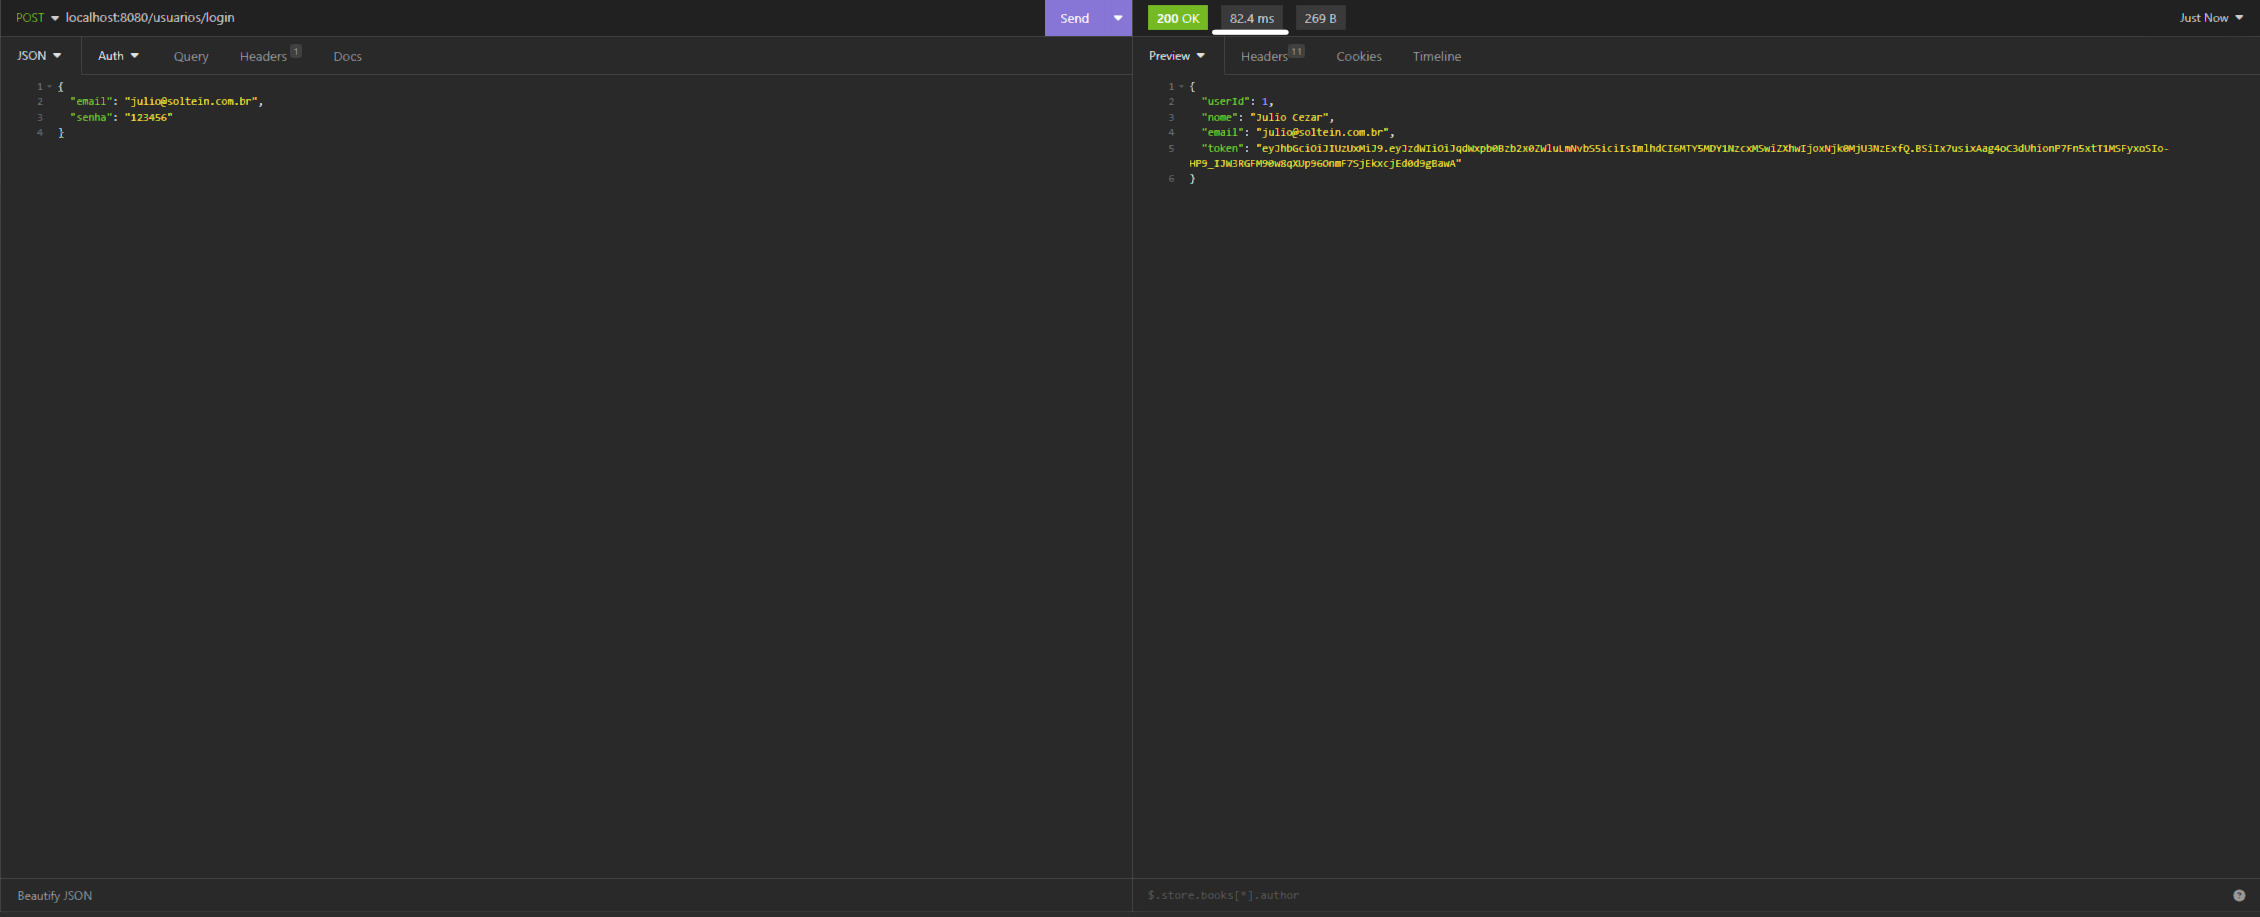
\includegraphics[width=1\textwidth]{desempenho.png}
    \caption{Tempo de resposta para acesso ao sistema. 82.4ms.}
    \label{fig:Tempo de resposta para acesso ao sistema. 82.4ms.}
 \end{figure}

 \chapter{Avaliação crítica dos resultados}

 De acordo com a proposta do projeto, podemos verificar que os requisitos não funcionais foram atendidos e validados com sucesso, mas há margem para melhorias como por exemplo em relação a integração com 
 operadora de pagamento online, deve-se focar na parte de segurança, fazendo um estudo mais aplicado nas opções de mercado antes de se optar por alguma.

 \noindent
 \begin{tabular}{|>{\raggedright\arraybackslash}p{4cm}|>{\raggedright\arraybackslash}p{10cm}|}
    \hline
    \cellcolor[gray]{0.8}Ponto Avaliado & \cellcolor[gray]{0.8}Descrição \\
    Arquitetura MVC & A utilização do padrão MVC permitiu que as responsabilidades do sistema fossem separadas de forma clara, isto irá facilitar a manutenção e evolução do mesmo. No entanto poderão surgir desafios em relação a manter a organização em camadas na medida que a equipe crescer, exigindo uma maior coordenação do desenvolvimento.\\
    \hline
    Usabilidade & Ao utilizar o Material Angular mantemos a padronização dos componentes de interface, e utilizamos recursos já utilizados em diversos aplicativos de software,
    isto permite manter uma facilidade de aprendizado para o usuário além de compatibilidade com diferentes resoluções. Como no desenvolvimento em camadas, a utilização do Material Angular
    requer que a equipe mantenha-se no propósito de utilizar o mesmo, sendo necessário novamente uma boa coordenação de equipe.\\
    \hline
    Segurança & No quesito de segurança garantimos a proteção de dados sensíveis através de criptografia e controle de acesso adequado. Mas ainda é necessário
    se atentar a outros quesitos como na questão de pagamentos online no que se refere a dados de cartão e também ao armazenamento do token de acesso.\\
    \hline
    Interoperabilidade & Ao utilizarmos o padrão RESTful que é amplamente aceito nos permitirá integra com a grande maioria de sistemas. Caso venha a ser 
    necessário se conectar a sistemas que utilizam padrão SOAP, a tecnologia Spring fornece facilitadores, mas mesmo nessa condição a manutenção de diferentes padrões poderá
    ser um complicador para a equipe de desenvolvimento.\\
    \hline
    Desempenho & Ao atender o requisito de desempenho tornamos a experiência para o usuário mais fluida, entretanto é necessário manter um monitoramento do sistema 
    e avaliar a necessidade futura de crescimento da infra-estrutura tanto vertical como horizontalmente.\\
    \hline
 \end{tabular}

 \chapter{Conclusão}

 Com a finalização deste trabalho podemos verificar o quão importante é a parte de definição arquitetural de um sistema. Através da avaliação 
 podemos identificar pontos que requerem uma atenção maior e uma maior cautela ao escolher um fornecedor, como por exemplo no quesito de pagamento online 
 e também no desempenho do sistema que requer tanto uma validação melhor por parte de segurança quanto um monitoramento das necessidades futuras.

 A arquitetura adotada, baseada no padrão MVC, mostrou-se uma escolha sólida, proporcionando uma 
 estrutura organizada e modular que facilitará a manutenção e a evolução do sistema. No entanto, enfrentaremos
 desafios em relação à integração entre as camadas, exigindo cuidados no gerenciamento de dependências.

 A decisão de padronizar comunicações com sistemas externos utilizando RESTful e JSON contribuirá
 para a interoperabilidade do sistema.

 Em resumo, a definição cuidadosa da arquitetura, aliada a uma avaliação crítica dos trade-offs, resultou em uma 
 arquitetura robusta e eficiente. A busca por uma arquitetura bem equilibrada é um processo contínuo que 
 impulsiona o sucesso do sistema, atendendo às necessidades dos usuários e permitindo sua evolução de 
 forma sustentável.

\chapter{Repositórios}

Abaixo os repositórios utilizados para salvar as informações do projeto integrado.
\\\\
\noindent
Código LATEX para geração do artigo.\\
\href{https://github.com/soltein/TCC}{https://github.com/soltein/TCC}
\\\\
Código Back End Java.\\
\href{https://github.com/soltein/Arquitetura_Software_PucMinas}{\url{https://github.com/soltein/Arquitetura_Software_PucMinas}}.
\\\\
Código Front End Angular\\
\href{https://github.com/soltein/frontend-arquitetura-pucminas}{https://github.com/soltein/frontend-arquitetura-pucminas}

\chapter{Vídeo Apresentação}

Vídeo de apresentação final do projeto. \\

\href{https://youtu.be/hxmr67Iwvps}{https://youtu.be/hxmr67Iwvps}

\bibliographystyle{plain}
\bibliography{bibliografia}
\end{document}